% this file is called up by thesis.tex
% content in this file will be fed into the main document
\chapter{Code/Manuals/Publications}
% top level followed by section, subsection


%%%%%%%%%%%%%%%%%%%%%%%%%%%%%%%%%%%%%%%%%%%%%%%%%%%%%%%%%%%%%%%%%%
\section{Simulations with XFLR5}
\label{Simulaciones con XFLR5}
XFLR5 is an open source software widely used for aerodynamic analysis and aircraft design.
%
It was developed mainly by Mark Drela, a leading aerospace engineer and professor at the Massachusetts Institute of Technology (MIT). His experience in aerodynamics and aircraft design was fundamental to the creation of this tool.
%
The development of XFLR5 began in the 1990s, which means it has been in development and evolution for several decades. This has allowed the tool to mature and become a reliable option for aircraft engineers and designers.
%
 XFLR5 is distributed under an open source license, which means that the software is free and its source code is available for anyone to examine, modify and distribute. This has fostered an active community of users and developers who contribute to its continuous improvement. It specializes in aerodynamic analysis of aircraft and gliders. It offers key features such as aerodynamic coefficient calculation, polar curve generation, flight simulation, aerodynamic profile optimization and more. 
\begin{figure}[h]
    \centering
    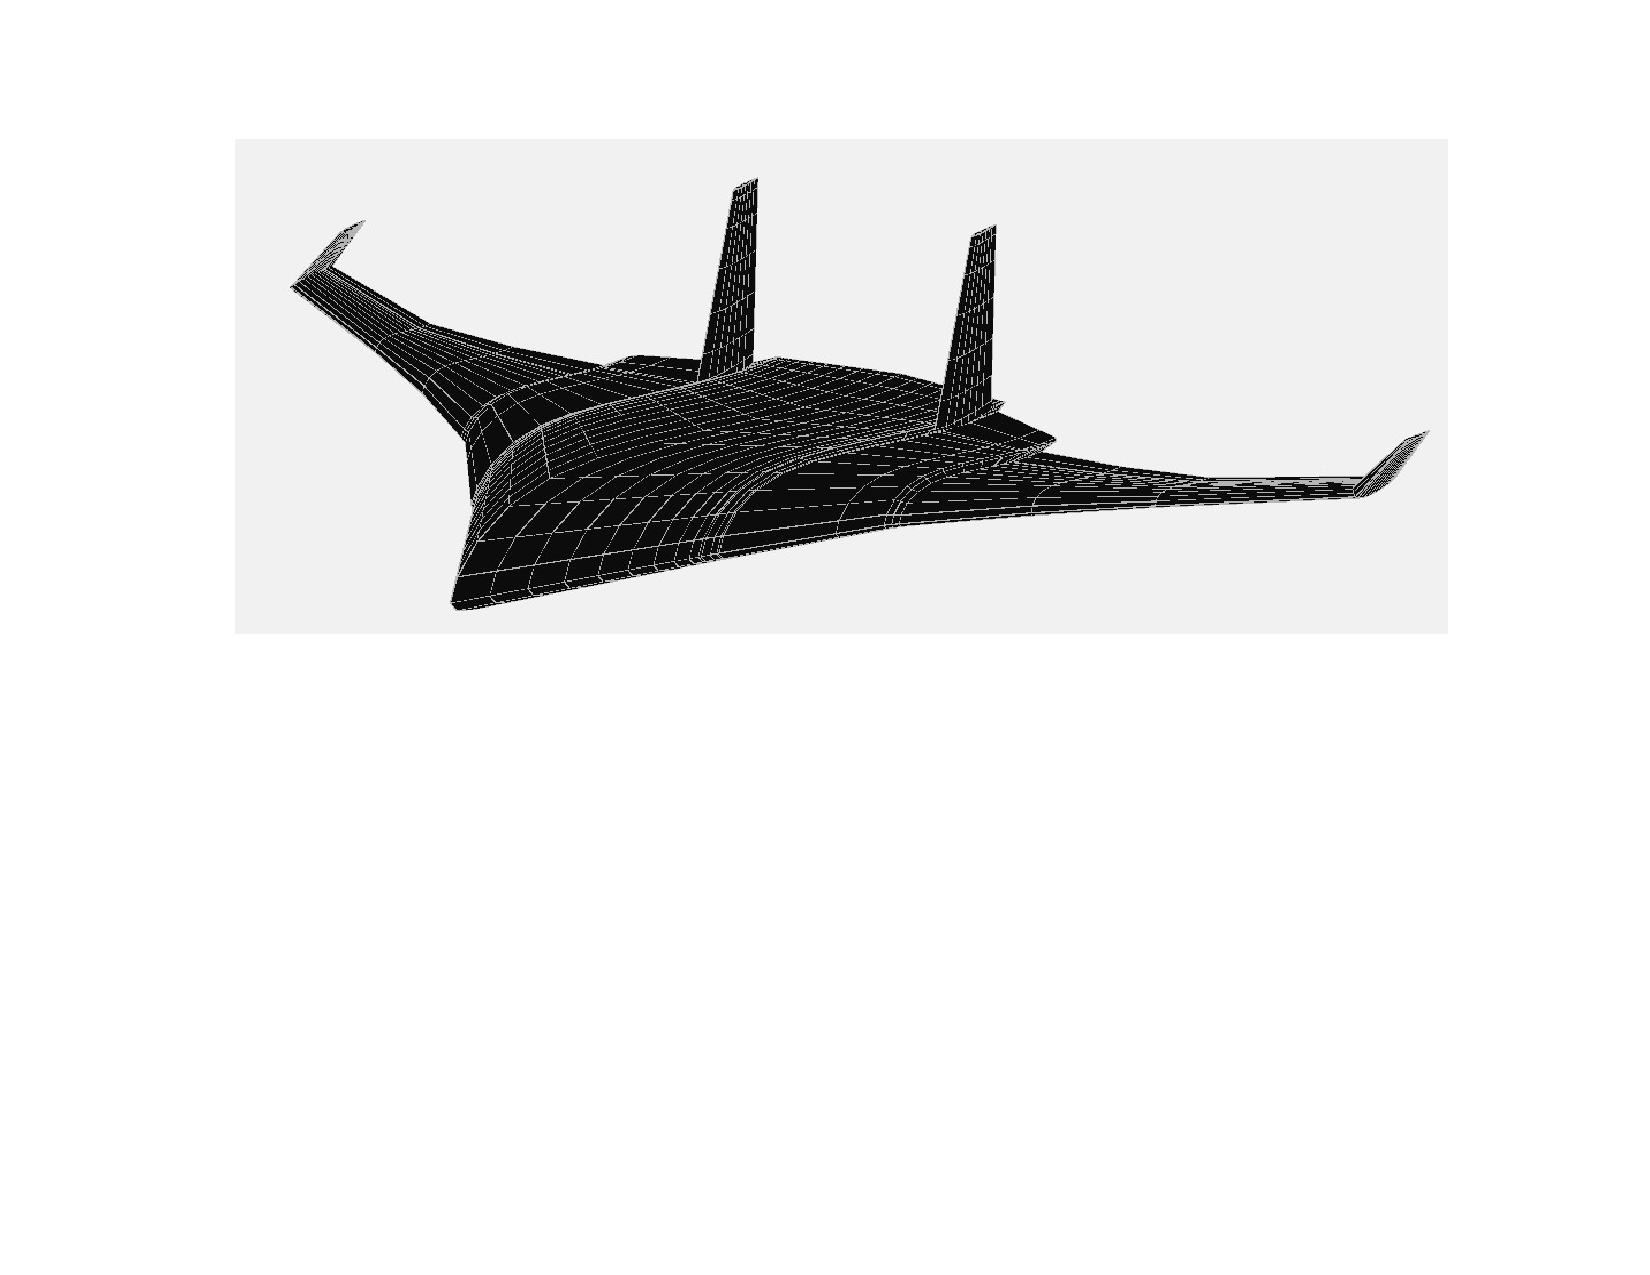
\includegraphics[scale=0.65]{Capitulo3/figs/paneles ehekatl_cropped.pdf}          
    \caption{Panel mesh for aerodynamic simulations}
    \label{Malla de paneles para simulaciones aerodinámicas}
\end{figure}

  Its history and focus on open source make it a valuable tool for the aerospace engineering community.
%
In the figure \ref{Malla de paneles para simulaciones aerodinámicas}, we observed EHEKATL BWB G-33 and the mesh considered in panels. In the table \ref{EHEKATL BWB G-33 ficha geometrica} We mentioned that 644 panels for our meshing. XFLR5 has three numerical methods for the solution of aerodynamic analysis. 
\begin{itemize}
    \item \textbf{Theory of the line of support} It is a simplified model that is used to understand and analyze the aerodynamics of a wing, especially in the context of finite wings (wings with a limited wingspan rather than infinite wings).You can model the aerodynamics of a wing by dividing it into segments, each treated as a separate aerodynamic profile.These segments are connected along the wing's wingspan, forming a continuous line or curve known as a "support line."Each segment generates individual support based on its local angle of attack and the characteristics of the aerodynamic profile.The Sustainability Line Theory in XFLR5 allows you to approximate the sustained and induced resistance of a finite wing.It is a valuable tool to analyze the performance of aircraft wings in the real world.
    \item \textbf{Horseshoe vortexes} A horseshoe vortex is a complex flow pattern that occurs near the tips of the wings of an aircraft or other supporting bodies. When an aircraft generates support, it creates a pressure difference between the top and bottom surfaces of its wings. This pressure difference induces air flow from the high pressure region below the wing towards the low pressure region above. Near the tips of the wings, this flow is rolled up and forms a vortex pattern that resembles a horseshoe. This horseshoe vortex is a significant contributor to induced resistance. Understanding the presence and behavior of the horseshoe vortex is crucial for aircraft design and aerodynamic optimization. Engineers seek to minimize the intensity of these vortexes to reduce resistance and improve efficiency.
    \item \textbf{Invalid Vortex} XFLR5 does not directly model annular vortexes, as they are typically associated with stele turbulence and aircraft interaction in real-world scenarios. However, the software can provide information about flow behavior near the wing tips and leak edges that can contribute to the formation of annular vortexes. Although XFLR5 does not explicitly simulate annular vortexes, it can help you understand the flow patterns and conditions that could lead to their formation. This knowledge can guide you in the design of wings and aircraft to minimize the impact of stele turbulence.
\item  \textbf{Paneles 3D} In the context of XFLR5 and the aerodynamic analysis of aircraft, the "3D panels" refer to a numerical technique that breaks down the wing surface and aircraft into a series of two-dimensional elements (panels) representing parts of the surface. These 3D panels can be considered as flat surfaces that roughly follow the shape of the wing and aircraft in three dimensions. Each 3D panel has associated aerodynamic properties, such as angle of attack, curvature, space position and aerodynamic coefficients. XFLR5 uses this 3D panel decomposition to calculate the aerodynamic forces and moments acting on the aircraft based on flight parameters and control settings.3D panel methods are an efficient way to perform detailed aerodynamic analyses of an aircraft, taking into account three-dimensional geometry and flight conditions.
\end{itemize}

The stability analysis of XFLR5 is based on the solution of the linear motion equations of an aircraft in response to small disturbances. When the stability and control analysis is performed to also obtain the coefficients of the ACS, the main limitation is that in this case the simulation does not consider viscous drag. We can define the following: \textbf{limitaciones} in the use of XFLR5:
%
1) Potential Flow Models: XFLR5 is based on potential flow models, which means that it does not solve the complete Navier-Stokes equations, but is based on simplifications. This makes it suitable for analysis of aerodynamic wings and profiles at subsonic and transonic speeds, but is not suitable for analysis of supersonic or hypersonic flows.
%
2) Small Disturbation Approach: XFLR5 assumes that the aircraft-induced disturbances in the flow are small, which is valid for most conventional aeronautical applications. However, it is not suitable for the analysis of high speed or high manoeuvrability aircraft, such as supersonic combat aircraft.
%
3) Simplifications in Geometry: The software uses a series of geometrical simplifications, such as two-dimensional wing profiles and straight wing models. This may limit your ability to model complex geometries or variable wing effects. 
%
4) Limitations on Operation Conditions: XFLR5 is more suitable for analysis of subsonic and transonic operating conditions. It is not the appropriate tool for analysis of hypersonic aircraft or rockets.
%
5) Sensitivity to Entry Data: The accuracy of simulations in XLR5 can depend to a large extent on the quality of input data, such as aerodynamic profiles and flow properties. Results may vary if data is not accurate or if important information is lacking.
%
6) Limited Analysis Capabilities: Although it is useful for aerodynamic wing and profile analysis, XFLR5 does not have the most advanced analysis capabilities that offer complete Computational Fluid Dynamics (CFD) tools. It cannot capture complex three-dimensional flow effects, advanced stability and control effects or complex air-to-air interactions.
%
7) It is not a Final Design Tool: XFLR5 is useful for conceptual design and preliminary analysis, but it is not designed for detailed aircraft design and analysis at the final engineering level. It is a valuable tool for the initial design phase, but designers often resort to more specialized tools for further analysis and validation. 
%
8) Accuracy in viscous trawling: XFLR5 is mainly based on methods of potential analysis and is therefore more suitable for calculating support and induced trawling (associated with support). However, it has limitations in the precise calculation of viscous trawling, which is the drag related to the friction of viscous flow on the surface of a wing. XFLR5 uses a simplified viscous trawl model that assumes that the flow is incomprehensible and that the boundary layer is thin. This can lead to inaccuracies in the calculation of drag in certain cases, especially in configurations where the boundary layer is significant or in high speed aerodynamic profiles.It is designed primarily for two-dimensional analysis and, although it can handle 3D configurations, it is not as accurate for highly three-dimensional cases or with complex 3D effects.Studies of wings in the form of swallow rope or wings with very irregular geometries may present challenges.To improve the accuracy of the viscous drag calculation, XFLR5 may depend on experimental data or drag coefficients provided by the user.This means that the accuracy of the viscous drag calculation may depend on the quality and availability of experimental data.

%%%%%%%%%%%%%%%%%%%%%%%%%%%%%%%%%%%%%%%%%%%%%%%%%%%%%%%%%%%%%%%%%%
\section{Modelling of the EHEKATL BWB with Thrust-Vector Control}
\label{modelado TVC}

The \textbf{Thrust Vector Control } through two servo-mechanisms of an articulated nozzle generates moments of pitching $\delta_{\theta}$ and yaw $\delta_{\psi}$, with a moment of arm according to

\begin{equation}
\label{eq: momento brazo del vector de empuje}
    l_T = x_{cg} - x_T
\end{equation}


where $x_{cg}$ is the centre of gravity of the aircraft, where the external forces operate; and $x_T$ is the axial axis of the TVC with respect to the origin of the propulsion reference system and vector thrust control.  


\begin{figure}[h]
\centering
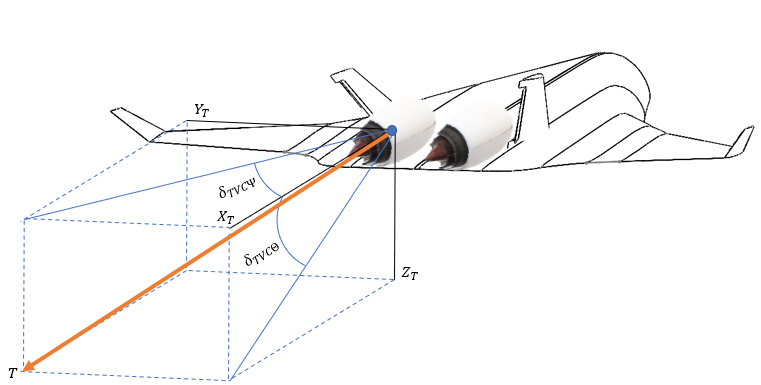
\includegraphics[scale=0.7]{Capitulo3/figs/4 13.png}
\caption{Vector Thrust Control Forces and Moments }
\label{fig: fuerzas y momentos del control de empuje vectorial}
\end{figure}


Now let's break down the forces and moments to identify the application and equation of the thrust vector on each axis. 

\begin{figure}[h]
\centering
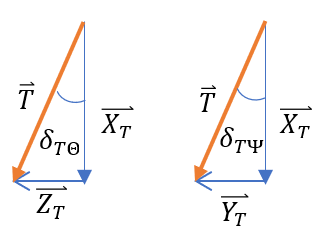
\includegraphics[scale=0.8]{Capitulo3/figs/4 14.png}
\caption{Components of vector thrust control }
\label{fig: componentes del control de empuje vectorial}
\end{figure}

The transformation generated by the moments of the TVC $\delta_{TVC \Theta}, \delta_{TVC \Psi}$ equals the moments generated in the centre of gravity of the aircraft $M_T, N_T$. 

Given the deflection of $\delta_{TVC \Theta}$ for the pitching moment (first triangle from left to right), shown in \ref{fig: componentes del control de empuje vectorial}, we defined the components of the thrust vector in the symmetric X-Z plane. 


\begin{equation}
    X_T = T C_{\delta_{T\Theta}}, \\
    Z_T = T S_{\delta_{T\Theta}}
\end{equation}

and the moment of pitching $M_T$ generated on the aircraft is 

\begin{equation}
    M_T = l_T Z_T
\end{equation}

We now define in a similar way the deflection of $\delta_{TVC \Psi}$ for the moment of yaw, according to the second triangle-rectangle. 

\begin{equation}
    X_T = T C_{\delta_{T\Psi}}, \\
    Y_T = T S_{\delta_{T\Psi}}
\end{equation}

the moment of yaw $N_T$ generated on the aircraft is 

\begin{equation}
    N_T = l_T Y_T
\end{equation}

The equations describing the behavior on each axis are shown below

\begin{align}
    X_{T} &= P_T C_{\theta} C_{\psi} \\
    Y_{T} &= P_T  S_{\psi}  \\
    Z_{T} &= P_T  C_{\psi} S_{\theta} 
\end{align}

Then the components of vector thrust control on the body axes are represented in the linear forces 
\begin{equation}
\begin{bmatrix}
X_{T} \\
Y_{T} \\
Z_{T}
\end{bmatrix}
=
T
\begin{bmatrix}
C_{\delta_{\Theta}} C_{\delta_{\Psi}} \\
S_{\delta_{\Psi}} \\
S_{\delta_{\Theta}}
\end{bmatrix}
\end{equation}

and at angular moments such as

\begin{equation}
\begin{bmatrix}
L_{T} \\
M_{T} \\
N_{T}
\end{bmatrix}
=
\begin{bmatrix}
0 \\
l_T Z_{T} \\
l_T Y_{T}
\end{bmatrix}
\end{equation}

According to our EHEKATL BWB configuration it is two engines that would act your TVC nozzles, so you have to consider the variables of each one, and then you set the linear moments

\begin{align}
    X_T &= T_{1} C_{\delta1_{\Theta}} C_{\delta1_{\Psi}} + T_{2} C_{\delta2_{\Theta}} C_{\delta2_{\Psi}} \\
    Y_T &= T_{1} S_{\delta1_{\Psi}} + T_{2} S_{\delta2_{\Psi}} \\
    Z_T &= T_{1} S_{\delta1_{\Theta}} + T_{2} S_{\delta2_{\Theta}}
\end{align}

and angular moments

\begin{align}
    L_T &= 0 \\
    M_T &= l_T(T_1 Y_{T1} + T_2 Y_{T2}) \\
    N_T &= l_T(T_1 Z_{T1} + T_2 Z_{T2})
\end{align}

%%%%%%%%%%%%%%%%%%%%%%%%%%
\section{Modeling of stability and control coupling terms}

In the non-linear coupled model it is possible to represent the coupling forces by means of stability derivatives, terms that are not normally developed. When we have the decoupled models we assume that the yawing and rolling movements do not produce any movement in pitch, and vice versa. One of the areas that are usually omitted during modeling in the flight dynamics is the modeling of the coupling forces. Among more than 20 coupled derivatives, two of them are the most important to represent the effects of lateral-directional and longitudinal dynamics, are the coupling derivatives of the sideslip angle. $C_{D_{\beta}}$ and the angle of rolling $C_{L_{\phi}}$. We can be negligent with the rest of derivatives and only consider these two. The reason why these two coefficients are sufficient to consider the complete non-linear coupled model are as follows: A pure longitudinal movement does not have a direct effect on lateral-directional mechanics, the main effect of directional motion on longitudinal mechanics is to increase the axial force (mainly the drag), and therefore reduces the longitudinal speed of the aircraft.

So the most significant value is the derivative. $C_{D_{\beta}}$. The main effect of lateral movement on longitudinal mechanics is to reduce the normal force (in other words the lift) of the aircraft. Therefore, the main derivative is $C_{L_{\phi}}$. 

Defining the coupling derivatives and updating the axial force and normal force the non-linear coupled modeling we obtain
\begin{gather}
    X = X_{\alpha} \alpha + X_{\dot \alpha}\dot \alpha + X_{u} u + X_{q} q + X_{\delta_{e}} \delta_{e} + X_{\beta} \beta \\
    Z = Z_{\alpha} \alpha + Z_{\dot \alpha}\dot \alpha + Z_{u} u + Z_{q} q + Z_{\delta_{e}} \delta_{e} + Z_{\phi} \phi
\end{gather}

and in accordance with \cite{Mohammad2020}. 

\begin{gather}
    X_{\beta} = (sign(\beta))q_{1}S_{vt}\frac{2}{\pi} \\
    Z_{\phi} = 0.1 mg (sign(\phi))
\end{gather}
Where the sign function is a sign convention. 

There are aerodynamic control surfaces that are considered over-acted. \textbf{ruddervator} and the \textbf{elevons}. The rudder-lift is used particularly when you have vertical stabilizers in V form, if both surfaces go in the same direction, either in one direction or in another we generate the moment of yawing, if the surfaces go in opposite directions but the same magnitude, we can generate the moment of pitching. Elevons are the main proposal for BWB aircraft due to the large number of control inputs in the trailing edge. If they move in the same direction and magnitude we generate nodding, if they do it in the same magnitude but different direction generate the moment of roll. Thanks to the notation of \cite{Beard2012} We can turn the rudders-lifts and elevons. 

\textbf{timones-elevadores}
\begin{equation}
\begin{bmatrix}
\delta_{e} \\
\delta_{r}
\end{bmatrix}
=
\begin{bmatrix}
1 & 1 \\
-1 & 1 
\end{bmatrix}
\begin{bmatrix}
\delta_{rr} \\
\delta_{rl}
\end{bmatrix}
\end{equation}

\textbf{elevons}
\begin{equation}
\begin{bmatrix}
\delta_{e} \\
\delta_{a}
\end{bmatrix}
=
\begin{bmatrix}
1 & 1 \\
-1 & 1 
\end{bmatrix}
\begin{bmatrix}
\delta_{er} \\
\delta_{el}
\end{bmatrix}
\end{equation}


Finally, we can declare the terms of the aerodynamic forces

\begin{align}
    X_A &= X_{u}u + X_{\alpha}\alpha + X_{\dot \alpha}\dot \alpha + X_{q}q + X_{\beta} \beta \\
    Z_A &= Z_{u}u + Z_{\alpha}\alpha + Z_{\dot \alpha}\dot \alpha + Z_{q}q + Z_{\phi} \\
    Y_A &= Y_{p}p + Y_{r}r + Y_{\beta}\beta + Y_{\dot \beta}\dot \beta  \\
    L_A &= L_{p}p + L_{r}r + L_{\beta}\beta + L_{\dot \beta}\dot \beta \\
    M_A &= M_{u}u + M_{\alpha}\alpha + M_{\dot \alpha}\dot \alpha + M_{q}q  \\
    N_A &= N_{p}p + N_{r}r + N_{\beta}\beta + N_{\dot \beta}\dot \beta
\end{align}

And the terms of the control forces

\begin{align}
    X_C &=  X_{\delta_{e}}\delta_{e} \\
    Z_C &=  Z_{\delta_{e}}\delta_{e} \\
    Y_C &=  Y_{\delta_{a}}\delta_{a} + Y_{\delta_{r}} \delta_{r}\\
    L_C &=  L_{\delta_{a}}\delta_{a} + L_{\delta_{r}} \delta_{r} \\
    M_C &=  M_{\delta_{e}}\delta_{e} \\
    N_C &=  N_{\delta_{a}}\delta_{a} + N_{\delta_{r}} \delta_{r}
\end{align}


In the external linear forces applied the terms of the air velocity vector $X_{\alpha} \alpha, Y_{\beta} \beta$ are usually used transformando $ X_{w} w, Y_{v} v$ the terms are considered. $ X_{\dot w} \dot w, Y_{\dot v} \dot v$ o $ X_{\dot \alpha} \dot \alpha, Y_{\dot \beta} \dot \beta$ as the case may be, although in the review of the art-state it is mentioned that these derivatives are usually small compared to the rest of the terms and we can be negligent with them. 



%%%%%%%%%%%%%%%%%%%%%%%
\section{Linearisation}
\label{linealizacion a}
For our linearization process we rely mainly on \cite{Etkin1996}, \cite{Lewis2016}, \cite{Schimdt1998}, \cite{USAF1988} and \cite{Mohammad2020}. 


In reality the non-linear model is who approaches the actual physical system of the aircraft. However, dealing with non-linear models is not a simple task. Linearization converts the non-linear model considering small deviations or disturbances from balance. Therefore, we can say that the linearization process cancels or ignores the non-linearities of the system. \cite{Mohammad2020}. G. H. Bryan (1911) introduced the idea of disturbances in forces and moments regarding a state of equilibrium $trim$ as a flight condition, and this approach is the most widely used so far \cite{Cook2007}. 


There are two basic methods for the linearization process: 
\begin{itemize}
    \item Jacobian Linealization (Taylor Series)
    \item Linearization by feedback (inverse dynamics)
\end{itemize}

The \textbf{Jacobian linearization} literally is negligent with the non-linearities of the model, while the \textbf{linearization by feedback} actively suppresses non-linearities \cite{Mohammad2020}.

It is well recognized that on an aircraft they can quickly change flight configurations (ascent-to-cruise transition, deceleration from descent to approach, deflate the \textit{}{flaps} and extend the landing gear, etc.), the linearization process must be considered with respect to a fixed flight condition \cite{Schimdt1998}. The subsequent linearization of motion equations allows us to determine the dynamic behavior of small amplitudes of the aircraft around a point of equilibrium or \textit{trim}Some important considerations for the disturbance analysis include:

\begin{itemize}
    \item The small movements of the dynamic will be initiated from the wing-level flight with the controls and the configuration of the aircraft's thrust in balance, this is known as \textbf{Static balance flight condition}.
    \item The body-axis will be aligned with the initial velocity vector, and by far, it will be known as the aircraft's axis-stability.
\end{itemize}

Any system of nonlinear equations can be linearized at a point of equilibrium. Linearization is only valid in the vicinity of the point of equilibrium. The point of equilibrium does not have acceleration, that is, the velocity is constant. Some flight operations at points of equilibrium are: 
\begin{itemize}
    \item Cruise flight with constant speed
    \item Promotion with constant speed
    \item Round with constant speed
\end{itemize}

Takeoff and landing have no equilibrium conditions, since the air speed is not constant. The linear system satisfies the property of overlap and homogeneity. 

A general form of a linear equation is $y=mx$, where $m$ is referred to as the slope and is a constant number. A linear term has degree one in the dependent variable and its derivative. A linear equation consists of a sum of linear terms. \cite{Mohammad2020}. Linearization then around a point of equilibrium can be achieved in two ways:
\begin{itemize}
    \item Using Taylor Series
    \item Substituyendo directamente
\end{itemize}

The usual procedure is to assume that aerodynamic forces and moments are dependent on disturbed motion variables and their derivatives only.  

The Taylor series expresses a sum function of each of the motion variables or their derivative. Since the motion variables are $u,v,w$ and $p,q,r$, each of these terms would be a function $f_i$, and exemplifying on the axial axis with the term $X$ We'd get: 

\begin{equation}
    X = X_{e} + (\frac{\partial X}{\partial u}u+\frac{\partial^2 X}{\partial^2 u}\frac{u^2}{2!}+\frac{\partial^3 X}{\partial^3 u}\frac{u^3}{3!} + ...)
\end{equation}

and this series applies for each function of motion variable, linear and angular, in its first derivative and of higher order, where the first term is a constant $X_{e}$. 

Since the theory of small perturbations considers these perturbations within the vantage point of equilibrium, the movement of variables is small, and for all practical cases only the first-order term in each of the series is significant. $ \dot \alpha$ o $\dot w$. On many occasions the value of this term is small compared to those of first order and by simplicity it could be omitted. 

Then we would define the derivatives of stability of the linear system such that 

\begin{align}
    X_a &= X_u u + X_{w}w + X_q q + X_{G}G \\
    Y_a &= Y_{v}v + Y_{p}p + Y_{r}r + Y_{G}G \\
    Z_a &= Z_u u + Z_{w}w + Z_q q + Z_{G}G  \\
    L_a &= L_{v}v + L_{p}p + L_{r} \\
    M_a &= M_u u + M_{w}w + M_q q \\
    N_a &= N_{v}v + N_{p}p + N_{r}r
\end{align}

and the terms of the control derivatives would be defined as
\begin{align}
\label{eq: entradas de control lineal}
X_c &= \textcolor{RoyalBlue}{X_{\delta_T} \delta_T}  + \textcolor{RoyalBlue}{X_{\delta_{e1}} \delta_{e1}} + \textcolor{RoyalBlue}{X_{\delta_{e2}} \delta_{e2}}  \\
Y_c &= \textcolor{RoyalBlue}{Y_{\delta_T} \delta_T}  + \textcolor{RoyalBlue}{Y_{\delta_{a1}\delta_{a1}}} + \textcolor{RoyalBlue}{Y_{\delta_{a2}\delta_{a2}}} + \textcolor{RoyalBlue}{Y_{\delta_{r}}\delta_{r}} \\
Z_c &= \textcolor{RoyalBlue}{Z_{\delta_T} \delta_T}  + \textcolor{RoyalBlue}{Z_{\delta_{e1}} \delta_{e1}} + \textcolor{RoyalBlue}{Z_{\delta_{e2}} \delta_{e2}}  \\
L_c &= \textcolor{RoyalBlue}{L_{\delta_{a1}\delta_{a1}}} + \textcolor{RoyalBlue}{L_{\delta_{a2}\delta_{a2}}} + \textcolor{RoyalBlue}{L_{\delta_{r}}\delta_{r}} \\
M_c &= \textcolor{RoyalBlue}{M_{\delta_{e1}} \delta_{e1}} + \textcolor{RoyalBlue}{M_{\delta_{e2}} \delta_{e2}} \\
N_c &= \textcolor{RoyalBlue}{N_{\delta_{a1}\delta_{a1}}} + \textcolor{RoyalBlue}{N_{\delta_{a2}\delta_{a2}}} + \textcolor{RoyalBlue}{N_{\delta_{r}}\delta_{r}}
\end{align}



The \textbf{direct technique} is based on the theory of small perturbations, where you substitute all independent variables, for example X with two terms $X_0,\Delta X(t)$, that of the initial equilibrium condition and the end of the disturbance. 

Since we assume the disturbances in $x$ small involves having only the linear terms. 

The angular variables will also be simplified with the theory of small perturbations, where the $sin(x)$ normalizes equal to x, and the $cos(x)$ equals one.  

Before linearization, the set of the six coupled motion equations will appear as:

\begin{gather}
    X_0 + \Delta X(t) - mg sin\theta = m(\dot u + qw - rv) \\
    Y_0 + \Delta Y(t) + mg cos\theta sin\phi = m (\dot v + ru - pw) \\
    Z_0 + \Delta Z(t) + mg cos\theta cos \phi = m ( \dot w + pv - qu) \\
    L_0 + \Delta L(t) = I_x \dot p - I_xz \dot r + (I_z - I_y)pr - I_xz pq \\
    M_0 + \Delta M(t) = I_y \dot q + (I_x - I_z) pr + I_xz (p^2 - r^2) \\
    N_0 + \Delta N(t) = I_z \dot r - I_xz \dot p + (I_y - I_x)pq + I_xz qr
\end{gather}


In a manner similar to declarations of forces and moments, linearization of time-dependent state variables will begin with a definition of initial equilibrium values plus the terms of small disturbances.

\begin{gather}
    u = u_0 + u(t) \\
    v = v_0 + v(t) = v(t) \\
    w = w_0 + w(t) = w(t) \\
    p = p_0 + p(t) = p(t) \\
    q = q_0 + q(t) = q(t)  \\
    r = r_0 + r(t) = r(t) \\
    \theta = \theta_0 + \theta(t) \\
    \phi = \phi_0 + \phi(t) = \phi(t) 
\end{gather}

The initial condition considered for the initial movement from the wing-level flight with the axle-body corresponding to the aircraft axis-stability allows the removal of the terms $v_0, w_0, p_0, q_0, r_0, \phi_0$ and is considered $u_0 = V_0$.

At zero time, when the movement of small disturbances is about to begin, the ratio of the above equations is simplified according to the static equilibrium conditions in the aircraft's forces and moments.

\begin{gather}
    X_0 - mg sin\theta_0 = 0 \\
    Y_0 = 0; (\phi_0) \\
    Z_0 + mg cos\theta_0 = 0 \\
    L_0 = M_0 = N_0 = 0
\end{gather}

According to the static equilibrium conditions, the axis $X$ has an initial condition since $u$ and $\theta_0$ are the components on this axis that can have an initial value other than zero, which by working in the symmetrical plane $X-Z$, the initial component on the Z axis would also be different from zero and proportional to the axis $X$. The term corresponding to the aerodynamic force on the Y axis is zero, given that flight at wing level and angle is considered $\phi_0=0$. This generates that in the components of the weight we take into account that $sin \phi_0 = 0$ and therefore the weight effect has no presence on the axis $Y$, and by side $cos \phi_0 = 1$ , which lailerons the term of $cos \theta_0$ for the weight component on the axle $Z$ and depending on the pitch angle. 

All moments are considered zero for this statically balanced flight condition. 

The force ratio involves trigonometric terms that can be linearized using angle considerations for small perturbations. 

The \textit{theorem of the sum and difference of angles} establishes the relation for the sum of two angles, as is the case in the theory of small disturbances given the initial condition angle and the angle considering the aerodynamic force. 

\begin{gather}
    sin(\theta_0 + \Delta \theta) = sin \theta_0 cos \Delta \theta + cos \theta_0 sin \Delta \theta \doteqdot sin\theta_0 + \Delta \theta cos \theta_0 \\
    cos(\theta_0 + \Delta \theta) = cos \theta_0 cos \Delta \theta - sin \theta_0 sin \Delta \theta \doteqdot cos\theta_0 - \Delta \theta sin \theta_0
\end{gather}

So, in short:

\begin{gather}
    sin\Theta = sin \Theta_0 + cos\Theta_0 \theta(t) 
\end{gather} 
for $\theta(t) << 1$, and
\begin{gather}
    sin\Phi = \phi(t)
\end{gather}
for $\phi_0 = 0$ and $\phi(t) << 1$
\begin{gather}
    cos \Phi = 1
\end{gather}

The demonstration of theorem \textit{the sum and difference of angles} is shown in the \textit{appendices}.

Then the linearized equations would be as follows:


\begin{gather}
    X_0 + \Delta X(t) + X_c - mg = m(\dot u + q_0 w + q w_0 - r_0 v - r v_0) \\
    Y_0 + \Delta L(t) Y_c + mg = m (\dot v + r_0 u + r u_0 - p_0 w - p w_0) \\
    Z_0 + \Delta Z(t) + Z_c + mg = m ( \dot w + p_0 v + p v_0 - q_0 u - q u_0) \\
    L_0 + \Delta L(t) = I_x \dot p + (I_z - I_y)(q_0 r + q r_0) \\
    M_0 + \Delta M(t) = I_y \dot q + (I_x - I_z) (p_0 r + p r_0) \\
    N_0 + \Delta N(t) = I_z \dot r + (I_y - I_x)(p q_0 + p_0 q)
\end{gather}

and we'd get 

\begin{gather}
    \dot u  = \frac{1}{m}(X_0 + \Delta X(t) + X_c) - g - (q_0 w + q w_0 - r_0 v - r v_0) \\
    \dot v = \frac{1}{m}(Y_0 + \Delta Y(t) + Y_c) + g -( r_0 u + r u_0 - p_0 w - p w_0) \\
    \dot w = \frac{1}{m}(Z_0 + \Delta Z(t) + Z_c) + g -( p_0 v + p v_0 - q_0 u - q u_0) \\
    \dot p = \frac{1}{I_x}(L_0 + \Delta L(t) + L_c) - (I_z - I_y)(q_0 r + q r_0) \\
    \dot q = \frac{1}{I_y}(M_0 + \Delta M(t) + M_c) - (I_x - I_z) (p_0 r + p r_0) \\
    \dot r = \frac{1}{I_z}N_0 + \Delta N(t) + N_c) - (I_y - I_x)(p q_0 + p_0 q)
\end{gather}

and if we consider the wind axle reference system, let us remember that 
\begin{gather}
    \dot V  = \frac{1}{mV}(X_0 + \Delta X(t) + X_c) - \frac{g}{V} - (q_0 \alpha + q \alpha_0 - r_0 \beta - r \beta_0) \\
    \dot \beta = \frac{1}{mV}(Y_0 + \Delta L(t) Y_c) + \frac{g}{V} -( r_0 u + r V_0 - p_0 \alpha - p \alpha_0) \\
    \dot \alpha = \frac{1}{mV}(Z_0 + \Delta Z(t) + Z_c) + \frac{g}{V} -( p_0 \beta + p \beta_0 - \alpha_0 V - \alpha V_0) \\
\end{gather}


%%%%%%%%%%%%%%%%%%%%%%%%%%%%%%%%%%%%%%%%%%%%%%%
\textbf{Linear Dynamic Longitudinal - 3GDL}\\
In longitudinal decouplement we consider only perturbations in the symmetric x-z plane.
\begin{align}
    X_0 + \Delta X(t) + X_c - mg &= m(\dot u + q_0 w + q w_0) \\
    Z_0 + \Delta Z(t) + Z_c + mg &= m ( \dot w + q_0 u - q u_0) \\
    M_0 + \Delta M(t) &= I_y \dot q
\end{align}

where the terms $X_0,Z_0, M_0$ represent the condition of balance and the terms $\Delta X(t),\Delta Z(t), \Delta M(t)$ On the basis of this criterion we can simplify the nomenclature knowing that the terms $X,Z,M$ by developing the terms of applied forces and moments we have to

\begin{gather}
    X_u u + X_w w + X_q q + \textcolor{RoyalBlue}{X_c} - mg = m(\dot u + q_0 w + q w_0) \\
    Z_u u + Z_w w + Z_q q + \textcolor{RoyalBlue}{Z_c} + mg = m ( \dot w + q_0 u - q u_0) \\
    M_u u + M_w w + M_q q + \textcolor{RoyalBlue}{M_c} = I_y \dot q
\end{gather}

where the control entries considered are

\begin{equation}
    \textcolor{RoyalBlue}{X_c = X_{\delta_{T}} + X_{\delta_e1} \delta_e1 + X_{\delta_e2} \delta_e2}
\end{equation}

clearing derivatives $\dot{u}, \dot{w},\dot{q},\dot{\theta}$ is obtained

\begin{align}
    \dot u &=\frac{1}{m}(X_u u + X_w w + X_q q + \textcolor{RoyalBlue}{X_c}) - g -q w_0  \\
    \dot w &= \frac{1}{m}(Z_u u + Z_w w + Z_q q + \textcolor{RoyalBlue}{Z_c}) + g + q u_0 \\
    \dot q &= \frac{1}{I_y}(M_u u + M_w w + M_q q + \textcolor{RoyalBlue}{M_c}) \\  
    \dot \theta &= q
\end{align}

and considering that the aircraft is in flight at then level

\begin{equation}
    \theta_{0} = w_0 = 0
\end{equation}

the equation of linear longitudinal dynamics can be simplified in its simplest form

\begin{align}
\label{lineal longitudinal cuerpo}
    \dot u &=\frac{1}{m}(X_u u + X_w w + X_q q + \textcolor{RoyalBlue}{X_c}) - g \\
    \dot w &= \frac{1}{m}(Z_u u + Z_w w + (Z_q + mu_0) q + \textcolor{RoyalBlue}{Z_c}) + g \\
    \dot q &= \frac{1}{I_y}(M_u u + M_w w + M_q q + \textcolor{RoyalBlue}{M_c}) \\  
    \dot \theta &= q
\label{lineal longitudinal cuerpo 1}
\end{align}

in the same way you can write the dynamic depending on the status variables of the attack angle and flight path


\begin{align}
    \dot u &=\frac{1}{mV}(X_u u + X_\alpha \alpha + X_q q + \textcolor{RoyalBlue}{X_c}) - \frac{g}{V} \\
    \dot \alpha &= \frac{1}{mV}(Z_u u + Z_\alpha \alpha + (Z_q + mu_0) q + \textcolor{RoyalBlue}{Z_c}) + \frac{g}{V} \\
    \dot q &= \frac{1}{I_y}(M_u u + M_\alpha \alpha + M_q q + \textcolor{RoyalBlue}{M_c}) \\  
    \dot \theta &= q
\end{align}

\begin{align}
    \dot u &=\frac{1}{mV}(X_u u + X_\alpha \alpha + X_q q + \textcolor{RoyalBlue}{X_c}) - \frac{g}{V} \\
    \dot \gamma &= -\frac{1}{mV}(Z_u u + Z_\alpha \alpha + (Z_q + mu_0) q + \textcolor{RoyalBlue}{Z_c}) - \frac{g}{V} \\
    \dot q &= \frac{1}{I_y}(M_u u + M_\alpha \alpha + M_q q + \textcolor{RoyalBlue}{M_c}) \\  
    \dot \alpha &= q - \dot \gamma
\end{align}

%%%%%%%%%%%%%%%%%%%%%%%%%%%%%%%%%%%%%%%%%%%%%
\textbf{Side-Directional Linear Dynamic Model - 3 GDL}


The linear lateral-directional dynamics of three degrees of freedom are then decoupled


\begin{gather}
    Y_0 + \Delta L(t) Y_c + mg = m (\dot v + r_0 u + r u_0 - p_0 w - p w_0) \\
    L_0 + \Delta L(t) = I_x \dot p + (I_z - I_y)(q_0 r + q r_0) \\
    N_0 + \Delta N(t) = I_z \dot r + (I_y - I_x)(p q_0 + p_0 q)
\end{gather}

considering the same criterion of nomenclature where it is part of a condition of equilibrium and we only consider the terms as peturbations of the system, the dimensional terms of partial derivatives of stability and control would be

\begin{gather}
    Y_\beta \beta + Y_q q + Y_r r + Y_c + mg = m (\dot v + r u_0 - p w_0) \\
    L_\beta \beta + L_q q + L_r r + L_c = I_x \dot p \\
    N_\beta \beta + N_q q + N_r r + N_c = I_z \dot r
\end{gather}

where the control entries are

\begin{equation}
    \textcolor{RoyalBlue}{Y_c = Y_{\delta_{a1}} \delta_{a1} + Y_{\delta_{a2}} \delta_{a2} + Y_{\delta_{r}} \delta_{r}}
\end{equation}

Clearing state derivatives and taking into consideration \cite{Schimdt1998} For the values of the dimensional coefficients. By simulating with these coefficients we obtained a better behavior in the signals of the control inputs. 

\begin{gather}
    \dot v = \frac{1}{m}(Y_\beta \beta + Y_q q + Y_r r + Y_c) + g - r u_0 \\
    \dot p = \frac{1}{I_x}(L_\beta' \beta + L_q' q + L_r' r + L_c') \\
    \dot r = \frac{1}{I_z}(N_\beta' \beta + N_q' q + N_r' r + N_c') \\
    \dot \phi = p
\end{gather}

and expressing in aerodynamic terms, and recalling that $u_0 = V_0 = V$

\begin{gather}
    \dot \beta = \frac{1}{mV}(Y_\beta \beta + Y_q q + (Y_r - mu_0) r + Y_c) + \frac{g}{V} \\
    \dot p = \frac{1}{I_x}(L_\beta' \beta + L_q' q + L_r' r + L_c') \\
    \dot r = \frac{1}{I_z}(N_\beta' \beta + N_q' q + N_r' r + N_c') \\
    \dot \phi = p
\end{gather}





%%%%%%%%%%%%%%%%%%%%%%%%%%%%%%%%%%%%%%%%%%%%%%%%%%%%%%%%%%%%%%%%%%%%%%%%%%%
\section{Wing area and required power}
\label{superficie alar y potencia requerida}

\textit{Matching plot} is a graphical approach that allows you to determine the \textbf{superficie alar} and the \textbf{potencia requerida}. 
\begin{itemize}
    \item[] Design objectives in \textit{Matching plot}
    \item Reference area ($S_{ref}$)
    \item Thrust requerido ($T$) o Potencia requerida ($P$)
\end{itemize}
%
Curves in \textit{matching plot} are the thrust-weight ratio or load power (axis of abcise) depending on the elongated load (axis of ordered). 

The \textbf{carga alar $\frac{W}{S}$} is the reason between the weight of the aircraft and the reference area or surface. The wing load indicates how much load the wing surface supports per unit area. 

The \textbf{thrust-weight ratio $\frac{T}{W}$} is the ratio that indicates how much thrust the aircraft can generate in relation to its total weight. The higher the thrust-weight ratio, the more capacity the aircraft will have to accelerate and maintain the flight in situations such as takeoff, ascent or maneuvers. 

The \textbf{weight-push ratio $\frac{W}{T}$} is the inverse relationship of $\frac{T}{W}$. Indicates how much weight the aircraft must bear for each push unit it produces. The lower the weight-push ratio, the more efficient the aircraft will be, as it will need less push to support its weight. 

The \textbf{power-to-weight ratio $\frac{P}{W}$} is the ratio indicating how much power is available to move a unit of weight. $\frac{P}{W}$ is desirable, as the aircraft indicates a higher acceleration and performance capacity. 

The \textbf{Power-weight ratio $\frac{W}{P}$} is the inverse relationship of $\frac{P}{W}$. Indicates how much weight must be supported for each available power unit. $\frac{P}{W}$, the aircraft will be more efficient as it will need less power to support its weight. 


The thrust-weight ratio $\frac{T}{W}$ usually used to determine the thrust of jet, turbofan or turbojet engines. $\frac{W}{P}$ is usually used in aircraft powered by propellers or propellers (\textit{turboprop o motores piston}).

\begin{itemize}
    \item Input speed at loss $ (\frac{W}{P} )_{V_s} = f_1 (\frac{W}{S}, V_s)$
    \item Maximum speed $ (\frac{W}{P} )_{V_{max}} = f_2 (\frac{W}{S}, V_{max})$
    \item Promotional status  $ (\frac{W}{P} )_{ROC} = f_2 (\frac{W}{S}, ROC)$
    \item Take-off runway length $ (\frac{W}{P} )_{S_{TO}} = f_3 (\frac{W}{S}, S_{TO})$
    \item Absolute service ceiling $ (\frac{W}{P} )_{ceiling_{a}} = f_3 (\frac{W}{S}, h_a)$
    \item Cruise service roof $ (\frac{W}{P} )_{ceiling_{c}} = f_3 (\frac{W}{S}, h_c)$
\end{itemize}

The speed of loss $V_s$, the maximum speed $V_{max}$the promotion regime $ROC$, the length of the takeoff runway $S_{TO}$, the absolute service ceiling $ceiling_a$ and the roof service on cruise $ceiling_c$ are the aircraft performance requirements shown in curves on the chart \textit{matching plot} according to the thrust or power required depending on the wing load. 
%
The equations (functions of each variable) are considered to \cite{Mohammad2020} and \cite{Sadraey2013}. 

\begin{table}[!h]
    \caption{Requirements of the Flight Mission}
    \centering
    \begin{tabular}{|c|c|c|}
    \hline
    \multicolumn{3}{|c|}{\textbf{Entry Parameters for Matching Plot} } \\
    \hline
    \multicolumn{3}{|c|}{\textbf{Flight Mission Requirements}} \\
    \hline
    Flight range & $12, 060 m$ & $39, 566.92 ft$ \\
    \hline
    Input speed at loss & $19 m/s$ & $62.33 ft/s$  \\
    \hline
    Take-off speed &  $22.8 m/s$ & $74.8 ft/s$ \\
    \hline
    Velocidad crucero & $27 m/s$ & $88.58 ft/s$ \\
    \hline
    Maximum speed & $35.1 m/s$ & $115.15 ft/s$ \\
    \hline
    Altitud & $2, 400 m$ & $7, 874 ft$\\
    \hline
    Track length for takeoff & $30 m$ & $3.28 ft$ \\
    \hline
    Promotional regime & $2.5 m/s$ & $8.2 ft/s$ \\
    \hline
    Absolute service ceiling & $120 m$ & $393.7 ft$ \\
    \hline
    Ceiling is serviced cruise & $90 m$ & $295.27 ft$ \\
    \hline
    \multicolumn{3}{|c|}{\textbf{Aerodynamic coefficients}} \\
    \hline
    Lift coefficient $C_L$ & \multicolumn{2}{|c|}{$0.2$} \\
    \hline
    Trawl coefficient $C_D$ & \multicolumn{2}{|c|}{$0.013$}  \\
    \hline
    Trawl coefficient at take-off $C_{D0}$ & \multicolumn{2}{|c|}{$0.025$} \\
    \hline
    Max. lifting coefficient. $C_{L_{max}}$ & \multicolumn{2}{|c|}{$0.48$} \\
    \hline
    Drag coefficient max. $C_{D_{max}}$ & \multicolumn{2}{|c|}{$0.028$}  \\
    \hline
    \multicolumn{3}{|c|}{\textbf{Geometry}} \\
    \hline
    Reference area & $1.4m^2$ & $15.06 ft^2$ \\
    \hline
    Appearance Ratio & \multicolumn{2}{|c|}{$3.9$} \\
    \hline
    \end{tabular}
    \label{Requerimientos de la misión de vuelo}
\end{table}
%%%%%%%%%%%%%%%%%%%
%\begin{table}[h]
%    \centering
%    \begin{tabular}{|c|c|c|}
%    \hline
%    \multicolumn{3}{|c|}{\textbf{Parámetros de operación para Matching Plot}} \\
%    \hline
%    \multicolumn{3}{|c|}{Desempeño aerodinámico} \\
%    \hline
%    Coeficiente de levantamiento $C_L$ & \multicolumn{2}{|c|}{$0.2$} \\
%    \hline
%    Coeficiente de arrastre $C_D$ & \multicolumn{2}{|c|}{$0.013$}  \\
%    \hline
%    Coeficiente de arrastre en despegue $C_{D0}$ & \multicolumn{2}{|c|}{$0.025$} \\
%    \hline
%    Coeficiente de levantamiento max. $C_{L_{max}}$ & \multicolumn{2}{|c|}{$0.48$} \\
%    \hline
%    Coeficiente de arrastre max. $C_{D_{max}}$ & \multicolumn{2}{|c|}{$0.028$}  \\
%    \hline
%    \end{tabular}
%    \caption{Desempeño aerodinámico}
%    \label{desempeño aerodinamico}
%\end{table}
%%%%%%%%%%%%%%%%%%%%%%%%
%\begin{table}[h]
%    \centering
%    \begin{tabular}{|c|c|c|}
%    \hline
%    \multicolumn{3}{|c|}{\textbf{Parámetros de operación para Matching Plot} } \\
%    \hline
%    \multicolumn{3}{|c|}{Geometría del sistemas aéreo no tripulado} \\
%    \hline
%    Área de referencia & $1.3 m^2$ & $3.22 ft^2$ \\
%    \hline
    %Relación de Aspecto & \multicolumn{2}{|c|}{$4.6$} \\
    %\hline
    %\end{tabular}
    %\caption{Geometría de referencia del sistema aéreo ni tripulado para matching %plot}
%    \label{geometria para matching plot}
%\end{table}

%
The requirements of the flight mission, aerodynamic coefficients and geometric parameters of EHEKATL BWB to develop \textit{Matching Plot} and select the design point are shown in the table \ref{Requerimientos de la misión de vuelo}.
%
A code was developed in PYTHON that shows the curves of \textit{Matching plot} based on the input requirements so that the user can determinate the design point.
%
The code shows the results for both propulsion systems (reaction and propeller engines) and for both systems units (English and International). 
%
\begin{table}[!h]
    \caption{Unit System in Matching Plot}
    \centering
    \begin{tabular}{|c|c|c|}
    \hline
    \multicolumn{3}{|c|}{Unit Systems in Matching Plot}\\
    \hline
     Variable & International System & English/British systems  \\
     \hline
     Velocidad    & $m/s$ & $ft/s$ \\
     Peso & $N$ & $lbf$ \\
     Area & $m^2$ & $ft^2$ \\
     Potencia & $Watt$ & $lb ft/s$ \\
     Densidad & $kg / m^3$ & $slug/ft^3$\\
     \hline
    \end{tabular}
    \label{US Matching plot}
\end{table}


\medskip
%%%%%%%%%%%%%%%%%%%%%%%%%%%%%%%%
\textbf{Maximum weight of take-off}

For the calculation of the maximum take-off weight the following classification is to be considered:
\begin{itemize}
    \item payload weight
    \item avionics weight
    \item energy weight
    \item empty weight
\end{itemize}


%%%%%%%%%%%%%%%%%%
The \textbf{payload weight} is the net load capacity carrying the unmanned aerial system and the target by which it was designed. In the case of EHEKATL BWB the payload weight is $0.28kg$ integrated graphics card $0.25kg$ and the camera with artificial vision capabilities with $0.03kg$. 

\textit{Graphic Card}\\
Jetson Nano is a small but powerful computer that allows you to work with Artificial Intelligence for example image sorting, object detection, segmentation and voice processing. All on an easy-to-use platform running to 5V. 
\textit{Especificaciones:}
Memory: 2Gb, CPU: Quad-core ARM A57 1.43Ghz, Camera: 2x MIPI CSI-2 DPHY wools, USB: 4x USB 3.0, USB 2.0 Micro-B, Dimensions: 100mm x 80mm x 29mm, Weight: 250g and Open access for CUDA. 

\textit{Camera AI}\\
The NVIDIA Jetson camera NANO HD AI 800M CSI interface IMX219 has a resolution of 1080p, and the field of view has an angle of 77$^{\circ}$. It can be used for neural networks, artificial vision, real-time image recognition, intelligent vehicles, among other applications. A transparent acrylic protector is included to fix and protect the camera. 
%
\begin{figure}[!h]
    \centering
    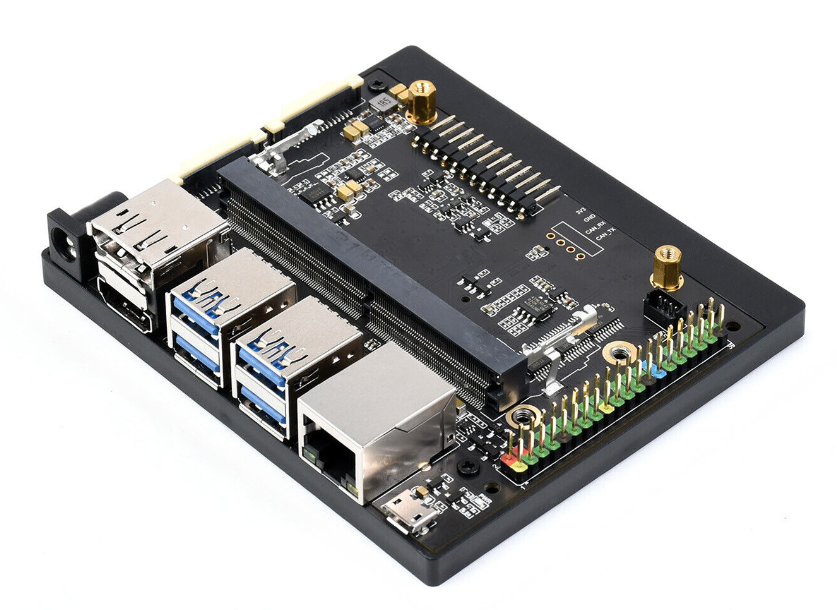
\includegraphics[scale=0.2]{Capitulo3/figs/3 22.png} 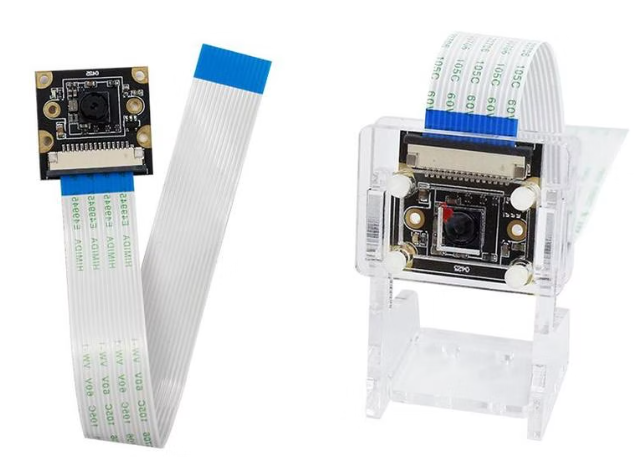
\includegraphics[scale=0.2]{Capitulo3/figs/3 23.png} 
    \caption{Payload: Jetson Nano and IA NVIDIA camera}
    \label{Carga útil:Tajera Jetson Nano y cámara IA NVIDIA}
\end{figure}

%%%%%%%%%%%%%%%%%%%%%
The \textbf{avionics weight} of EHEKATL BWB $0.225kg$. is integrated by the standard Pixhawk flight controller kit.

\textit{Auto-piloto} \\
Pixhawk is an open source flight control hardware. It runs with PX4 and Ardupilot environments.
\textit{Especificaciones}: 32 bit ARM Cortex M4 Processor running NuttX RTOS, 14 PWM/Servo outputs (8 with failure tolerances and manual override, 6 high power supported auxiliaries), Redundant power inputs and automatic switching, High power and multitone piezo audio indicator, Applications: Navigation and localization, research and education, control and stabilized systems, Frequency: 168 Mhz, RAM: 256 KB, Memory: 2MB Flash, Storage: SDCard port, Dimensions: 81.5x50x15.5mm, Weight: 38g, IMU: gyroscope, Accelerator and barometer; Standard kit: telemetry receivers, 4G TF card, security button, buzzer, PPM encoder, expansion plate I2C, 3 lines, M8N GPS, GPS support, 3DR power module and shock absorber. 

\begin{figure}[!h]
    \centering
    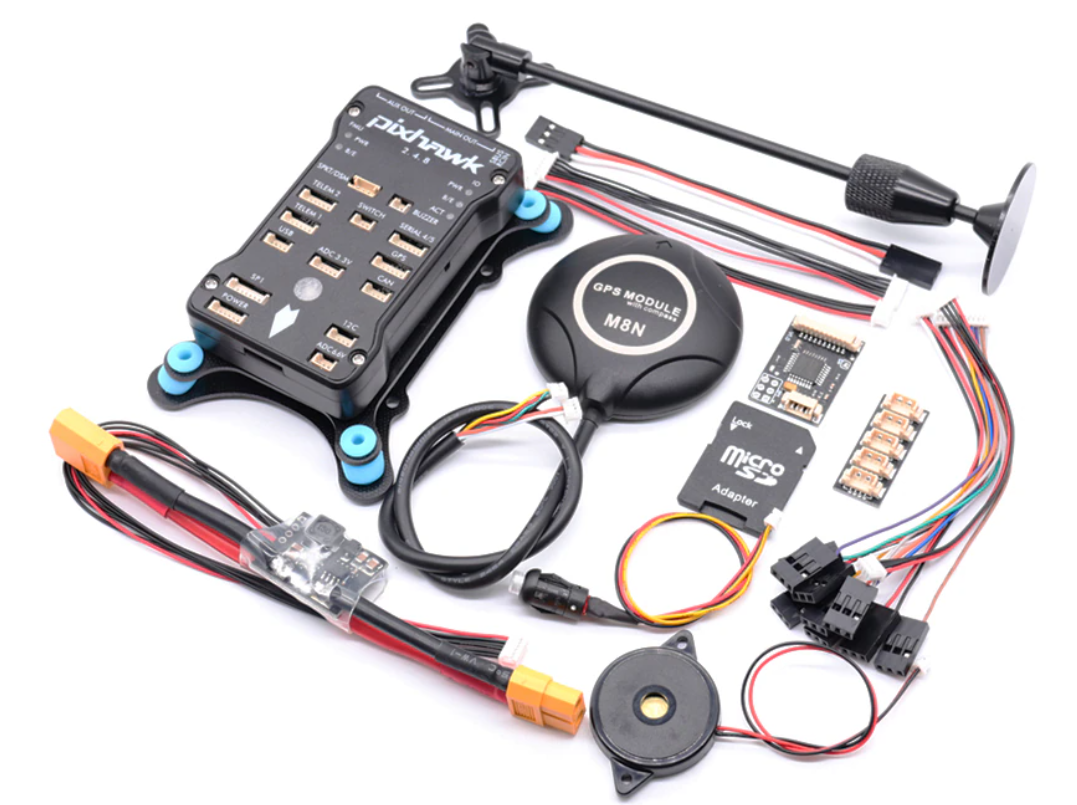
\includegraphics[scale=0.25]{Capitulo3/figs/3 17.png} 
    \caption{Avionics}
    \label{fig:enter-label}
\end{figure}

%%%%%%%%%%%%%%%%%%%%%%%%%%%%%%%%%%%%%%%
The \textbf{weight of the energy system} It can be analyzed in a different way: if fuel is consumed the specific fuel consumption ratio must be considered. For EHEKATL BWB we will consider electric batteries with the objective of not emitting combustion gases. With the implementation of batteries you also get simpleness in the maintenance. $0.359kg$ each piece, being a total of $0.718kg$ of the two batteries.

\textit{Battery} \\
A Zippy battery was selected with the following specifications: Capacity: 3300mAh, 4S1P/4/cellular 14.8V, Download 40C, 359g (considering all components), Dimensions 139x45x30mm, JST-XH plug balance and Discharge Plug: XT60.

\begin{figure}[!h]
    \centering
    
\includegraphics[scale=0.39]{Capitulo3/figs/3 15.png} 
    \caption{Energy}
    \label{Energía}
\end{figure}

The calculation of the power output $B_p$ of the batteries refers to the amount of electrical energy that the battery can provide to a charge within a certain period of time. 
\begin{equation}
\label{battery output power}
    B_p = n I V
\end{equation}
Where $n$ It's the number of batteries, $I$ the electrical current and $V$ the voltage. According to the selected Zippy battery we have the following features:
\begin{itemize}
    \item load capacity: 3300 mAh
    \item voltaje: 22.2 V
    \item consumption time: 1 hour
    \item No. of batteries: 2
\end{itemize}
Substituting for \ref{battery output power} We have to: 

\begin{gather}
     B_p = (2) (3300/1000) (22.2) \\
     B_p = 146.52 Wh
\end{gather}
Connecting the batteries in parallel we get an output power of $146.52 Wh$.

The energy density of the battery refers to the amount of energy that can be stored in a battery per unit of volume. 
\begin{equation}
    E_D = B_p E_c / m_b n
\end{equation}
where $E_c$ is the time of energy consumption in hours and  $m_b$ According to our two Zippy batteries we have to:
 \begin{gather}
    E_D = (146.52) (1) / (0.36) (2) \\
    E_D = 203.50 Wh/kg
\end{gather}

So an energy density of the energy system is established. $203.50 Wh/kg$.

For the fraction of the weight of the energy system with respect to the take-off weight we will establish the estimation of the following parameters: $C_L / C_D = 15.38$, an efficiency of the ductofan or propeller engines of  $\eta  = 0.81$ and a range of  $R= 12,060 m$.

\begin{gather}
    \frac{W_B}{W_{TO}} = 1.05 (\frac{g}{E_D \eta 3600} \frac{R}{C_L/C_D}) \\
    \frac{W_B}{W_{TO}} = 0.0136
\end{gather}

\medskip

The \textbf{empty weight} is composed of:
\begin{itemize}
    \item aero-estructura
    \item motores
    \item landing gear
    \item sistemas
\end{itemize}

So far we do not have dimensions in the geometry of EHEKATL BWB, therefore, the corresponding fraction of the empty weight relative to the maximum take-off weight cannot be calculated analytically. 

Based on historical data in order to apply a linear regression the fraction of the weight to the vacuum can be expressed the following relationship. 
\begin{equation}
\label{peso vacío equation}
    \frac{W_E}{W_{TO}}= a W_{TO} + b
\end{equation}


\begin{table}[!h]
    \centering
    \begin{tabular}{|c|c|}
    \hline
    a & b \\
    \hline
     $-4.6^-5$& $0.68$  \\
    \hline
    \end{tabular}
    \caption{Slope and intercept coefficients for the estimation of the empty weight of small-scale aircraft built in a workshop or house \cite{Sadraey2013}}
    \label{coeficientes del peso al vacío}
\end{table}

Substituting the values of \ref{coeficientes del peso al vacío} in \ref{peso vacío equation} tenemos: 

\begin{equation}
\label{peso vacío equation}
    \frac{W_E}{W_{TO}}= -4.6^-5 W_{TO} + 0.68
\end{equation}

The \textbf{maximum take-off weight} we can describe it intuitively as the sum of payload weights $W_{PL}$, the flight control system or avionics $W_{A}$, the energy system $W_{B}$ and the weight to the vacuum $W_{E}$:

\begin{equation}
    W_{TO} = W_{PL} + W_{A} + W_{B} + W_{E}
\end{equation}

The above equation can also be expressed considering the empty weight factors ($W_E/W_{TO}$) and energy system ($W_B/W_{TO}$) The suffix is usually used. \textit{B} for batteries and \textit{F} for fuel in the case of the fraction of the energy system. 
\begin{equation}
\label{peso de despegue fracc}
    W_{TO} = \frac{W_{PL}+W_{A}}{1-\frac{W_B}{W_{TO}}-\frac{W_E}{W_{TO}}}
\end{equation}

We update the value of $b$ in $0.78$ to obtain a greater take-off weight and allow us some slackness in later decisions of structure and manufacture. Substituting \ref{peso vacío equation} in \ref{peso de despegue fracc} e equal to zero we get a quadratic equation with respect to the take-off weight or maximum take-off weight:

\begin{equation}
\label{ecuación cuadrática de peso la vacío}
    -4.6^-5 W_{TO}^2 + (1-0.78-\frac{W_B}{W_{TO}})W_{TO} - (W_{PL}+W_{A})=0
\end{equation}

 
Solving the equation \ref{ecuación cuadrática de peso la vacío} and taking the positive root we calculate we get the following maximum takeoff weight:

\begin{table}[h]
    \centering
    \begin{tabular}{|c|c|c|}
    \hline
     \multicolumn{3}{|c|}{Maximum take-off weight $W_{TO}$} \\
     \hline
    $6.31 kg$ & $61.86 N$ & $13.91 lb$ \\
     \hline
    \end{tabular}
    \caption{Maximum take-off weight}
    \label{peso maximo de despegue}
\end{table}

According to the four weights that integrate the take-off weight for EHEKATL BWB the table is shown 
%%%%%%%%%%%%%%%%%%%%%%%%%%%%%%%%%%%%%%%%%%%%%%%%%%%%%%%%%%%%%%%%%%%%%%%%%%%%%%%%%%%%%%%%%%%%
\begin{table}[!h]
    \centering
    \begin{tabular}{|c|c|c|c|c|}
    \hline
    \multicolumn{5}{|c|}{Weight breakdown of EHEKATL BWB}\\
    \hline
     \textbf{$W_{TO}$} & \textbf{$6.31 kg$} & \textbf{$61.86 N$} & \textbf{$13.91 lb$} & $100 \% $  \\
     \hline
      $W_{PL}$ & \textit{$0.30 kg$} & \textit{$2.94  N$} & \textit{$0.66 lb$} & $ 4.75 \% $\\
      $W_{A}$  & \textit{$1.00 kg$} & \textit{$9.81  N$} & \textit{$2.20  lb$} &  $ 15.84 \% $  \\
      $W_{B}$  & \textit{$0.72 kg$} & \textit{$7.06  N$} & \textit{$01.59 lb$} &  $ 11.41 \% $ \\
      $W_{E}$  & \textit{$4.29 kg$} & \textit{$42.05  N$} & \textit{$9.45 lb$} &  $ 67.98 \% $ \\
    \hline
    \end{tabular}
    \caption{Breakdown and percentage of weights that integrate the take-off weight of EHEKATL BWB}
    \label{desglose y porcentaje de pesos}
\end{table}


The vacuum weight is considered based on the selected coefficients and only the project is used as an approximation at this stage.

\bigskip
%%%%%%%%%%%%%%%%%%%%%%%%%%%%%%%%%%%%%%%%%%%%%%%%%%%%%%%%%%%%%%%%%%%%%%%%
\textbf{Input speed at loss}\\
The loss speed refers to the minimum speed an aircraft must have before losing support and losing. Only helicopters and vehicles with vertical take-off capacity (\textit{VTOL}) are able to fly without a forward speed. The speed of entry in loss depends on the type of aircraft, its weight and the angle of attack. 

In the lifting force equation, as well as the speed of the aircraft decreases the lifting coefficient must increase, until finding the loss speed. An aircraft must be able to be in longitudinal equilibrium in the cruise flight condition and within the range of speeds ranging from the loss speed to the maximum speed. 

During the cruise flight at a loss of entry speed, the weight of the aircraft $W_{TO}$ must be balanced with the lifting force $L$. 
\begin{equation}
\label{lift}
    L = W_{TO} = \frac{1}{2} \rho V_s^2 S C_{L_{max}}
\end{equation}
Working the reference area on both sides of the equation \ref{lift} we get the first parameter for the selection of the design point with \textit{Matching Plot}. 
\begin{gather}
\label{velocidad de perdida}
    (\frac{W}{S})_{V_{s}} = \frac{1}{2} \rho V_s^2  C_{L_{max}} \\
    (\frac{W}{S})_{V_{s}} = \frac{1}{2} (0.9664) (19)^2 (0.48) \\
    (\frac{W}{S})_{V_{s}} = 83.74 N/m^2
\end{gather}
This result is general, both for jet engines and propela engines. 
%
The outcome in the international system of \textbf{$83.74 N/m^2$} is equivalent to \textbf{$1.75 lbf/ft^2$}. 
\begin{figure}[!h]
\centering
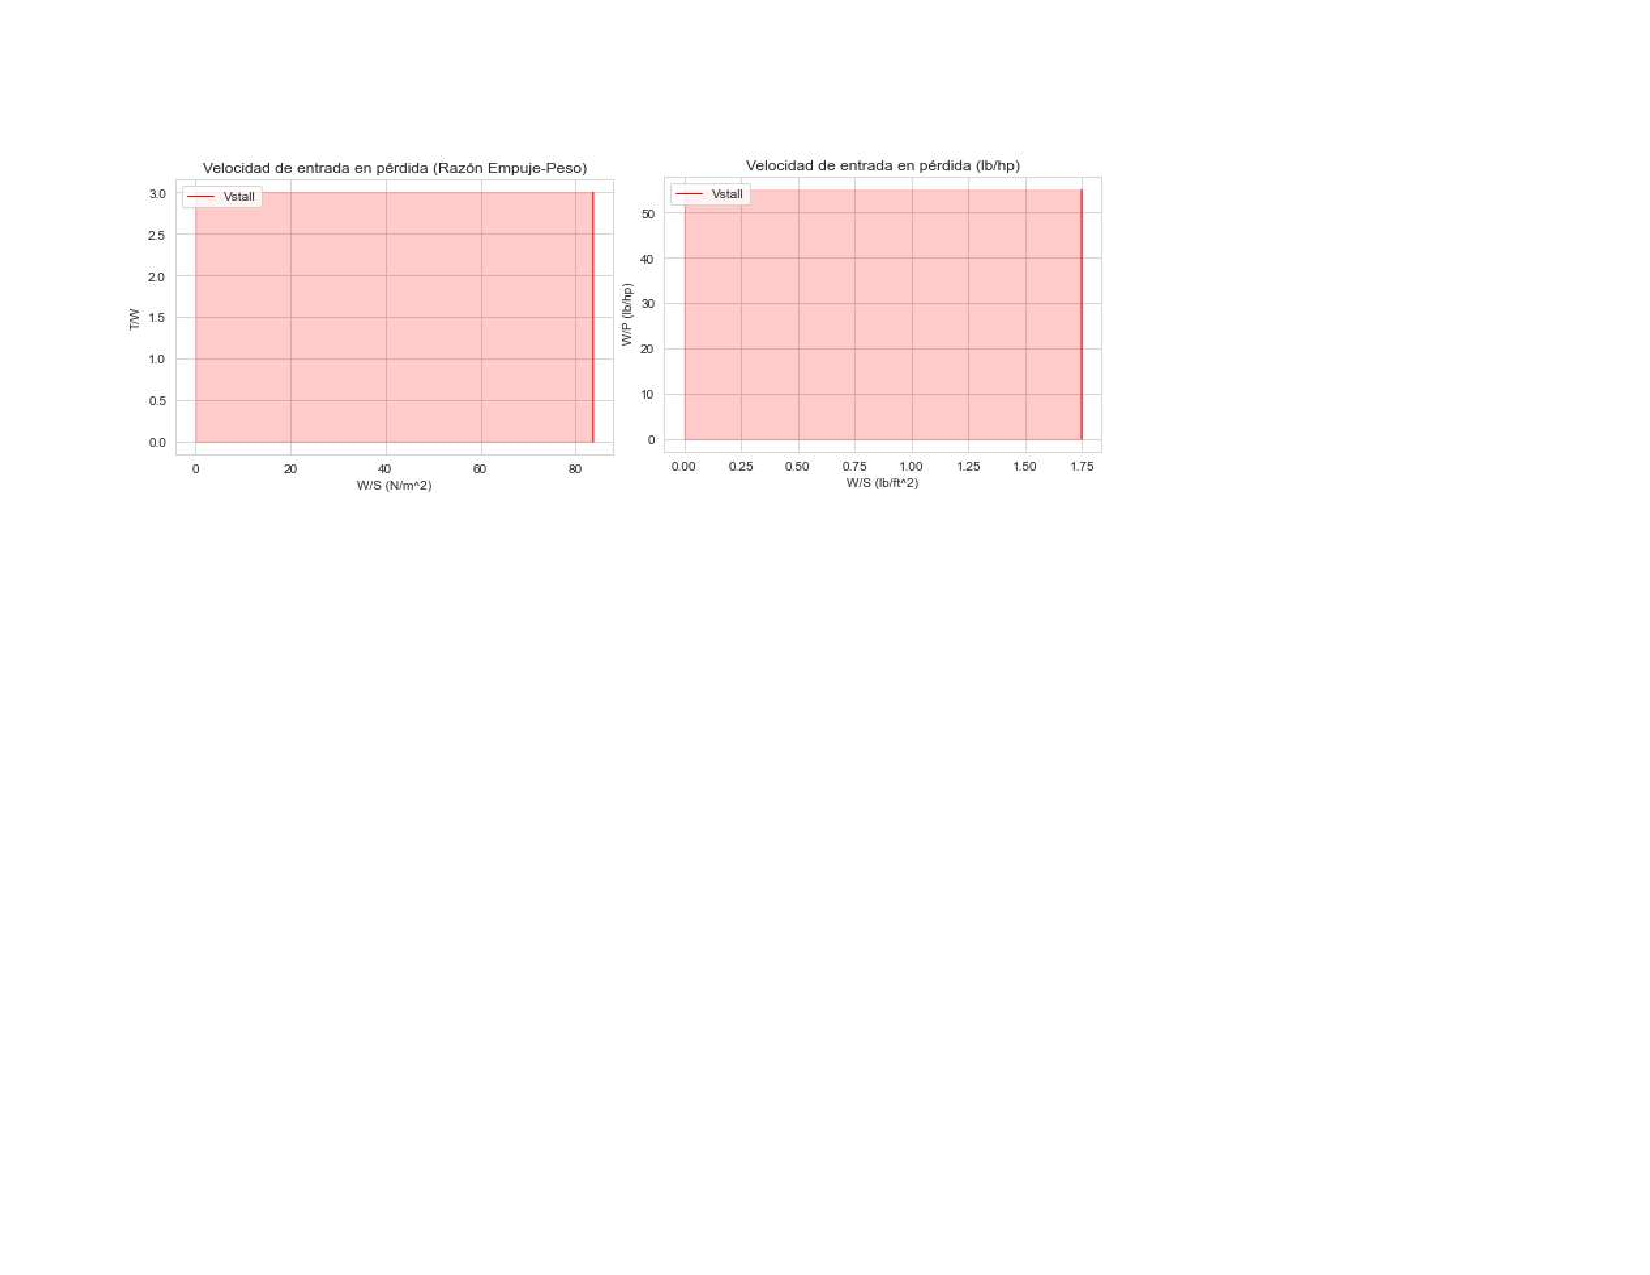
\includegraphics[scale=0.82]{Capitulo3/figs/Vstall_cropped.pdf}
\caption{Input speed at loss}
\label{Vstall}
\end{figure}

\bigskip
%%%%%%%%%%%%%%%%%%%%%%%%%%%%%%%%%%%%%%%%%%%%%%%%%%%%%%%%%%%%%%%%%%%%%%%%
\textbf{Maximum speed}

The maximum speed is another decisive factor in the schematization of \textit{Matching Plot}. For jet engines let us consider that the aircraft flies at its maximum constant speed at a specific altitude. The aircraft is in longitudinal equilibrium, therefore, the maximum power of the engines $T_{max}$ shall be equal to the maximum drag $D_{max}$ and weight $W_{TO}$ of the aircraft shall be equal to the lifting $L$:
\begin{gather}
    T_{max} = D_{max} \\
    W = L
\end{gather}

Where the lift and drag are defined as:

\begin{gather}
    D = \frac{1}{2} \rho V_{max}^2 S C_D \\
    L = \frac{1}{2} \rho V_{max}^2 S C_L
\end{gather}

It is important to mention that the thrust of the engines decreases as the altitude increases. The thrust varies with the speed of the air and the altitude. 

\begin{equation}
    T_{alt} = T_{SL} \frac{\rho}{\rho_0} = T_{SL} \sigma
\end{equation}

The Suffix $SL$ alludes to sea level. The density ratio is the density of the flight altitude relative to the density at sea level.

If we said the maximum thrust is equal to the maximum drag, then we can define the next equation. 

\begin{equation}
\label{empuje nivel del mar}
    T_{SL} \sigma = \frac{1}{2} V_{max}^2 S C_D
\end{equation}

The \textbf{drag coefficient} is divided into two main types: \textbf{zero-lifting $C_{D_0}$} and \textbf{lift-induced drag $C_{D_i}$}:

\begin{equation}
    C_D = C_{D_0} + C_{D_i} = C_{D_0} +  K C_{L}^2 
\end{equation}

where $K$ is the induced drag factor defined as:

\begin{equation}
    K = \frac{1}{\pi e AR}
\end{equation}

where $e$ is Oswald's efficiency factor in embarrassment, which usually goes from $0.7$ and $0.95$. 


The lift coefficient can be expressed according to weight. 

\begin{equation}
\label{levantamiento peso}
    C_{L} = \frac{2W}{\rho V_{max}^2 S}
\end{equation}

The \textit{zero-lifting coefficient $C_{D0}$} is another fundamental parameter in the calculations of \textit{matching plot}. It is also known as a parasite drag coefficient. It is a drag measurement generated by an object that moves through a fluid. This type of drag is also known as skin friction or viscous arratre. It is generated by the geometry, dimension and texture of the aircraft surface; and not by the production of support. Induced drag, also known as a support-induced drag factor, is a measure of the drag production relative to the lifting generation. 

\begin{table}[h]
    \centering
    \resizebox{14cm}{!} {
    \begin{tabular}{|c|c|c|}
    \hline
         & \textbf{Parasite Drag } & \textbf{Arrastre Inducido}\\
         \hline
      Peso   &  Not Influenced & Increases with weight gain\\
      Velocidad & Increases with speed increase & Decrease with speed increase\\
      Altitud & Decrease according to altitude  & Increase according to altitude\\
      Attack angle & Does not affect & Increases with increased angle of attack\\
      \hline
    \end{tabular}
    }
    \caption{Parasite Drag vs Induced Drag}
    \label{Arrastre parásito vs Arrastre inducido}
\end{table}

The equation for calculating the zero-lift coefficient in reaction engines is as follows:

\begin{equation}
    C_{D_0} = \frac{2 T_{SL_{max}} - \frac{4 K W^2}{\rho \omega V_{max}^2 S}} {{\rho_{0} V_{max}^2 S}}\\
\end{equation}

The equation for calculating the zero-lift drag coefficient with propeller engines is as follows:

\begin{equation}
    C_{D_0} = \frac{2 \frac{P_{SL_{max}} \eta_{P}}{V_{max}}  - \frac{4 K W^2}{\rho \omega V_{max}^2 S}} {\rho_{0} V_{max}^2 S} \\
\end{equation}

\medskip

Through algebra we develop the equation \ref{levantamiento peso} in \ref{empuje nivel del mar}, and clearing the term $\frac{T}{W}$ obtenemos:

\begin{equation}
    (\frac{T_{SL}}{W})_{V_{max}} = \rho_0 V_{max}^2 C_{D_{0}} \frac{1}{2 \frac{W}{S}} + \frac{2K}{\rho \sigma V_{max}^2} \frac{W}{S}
\end{equation}

The reason for the thrust loading $(\frac{T}{W})$ is a non-linear function with respect to the wing load $(\frac{W}{S})$. As the maximum speed is increased it also increases the rate of thrust-weight. The maximum speed is usually between a $20-30 \%$ above cruise speed. The region acceptable for the design point with jet engines is shaded above the curve in blue.

When we consider a propulsion system with propellers or propellers, the maximum power available in engines $P_{max}$ must be equal to the maximum power required $P_{req}$, which is the thrust multiplied by the maximum speed:

\begin{equation}
    P_{req} = \eta_{P} P_{max} = T V_{max}
\end{equation}

where the push $T$ must be equal to drag $D$. Entonces tenemos:

\begin{equation}
    \eta_{P} P_{SL} \sigma = \frac{1}{2} \rho V_{max}^2 S C_{D} =  \frac{1}{2} \rho V_{max}^3 S C_{D}
\end{equation}

By developing the above equation with the same considerations we did in the jet engine thrust, we get:

\begin{equation}
    (\frac{W}{P_{SL}})_{V_{max}} = \frac{\eta_{P}}{\frac{1}{2} \rho_{0} V_{max}^3 C_{D_{0}} \frac{1}{(\frac{W}{S})} + \frac{2K}{\rho \sigma V_{max}} (\frac{W}{S})}   
\end{equation}

In $\frac{W}{P}$ when the maximum speed value increases the load power $\frac{P}{W}$ This is because in the first term of the equation we have $V_{max}^3$. The acceptable region is below the curve, contrary to the calculation in Jet engines, see figure \ref{Vmax}.

\begin{figure}[!h]
\centering
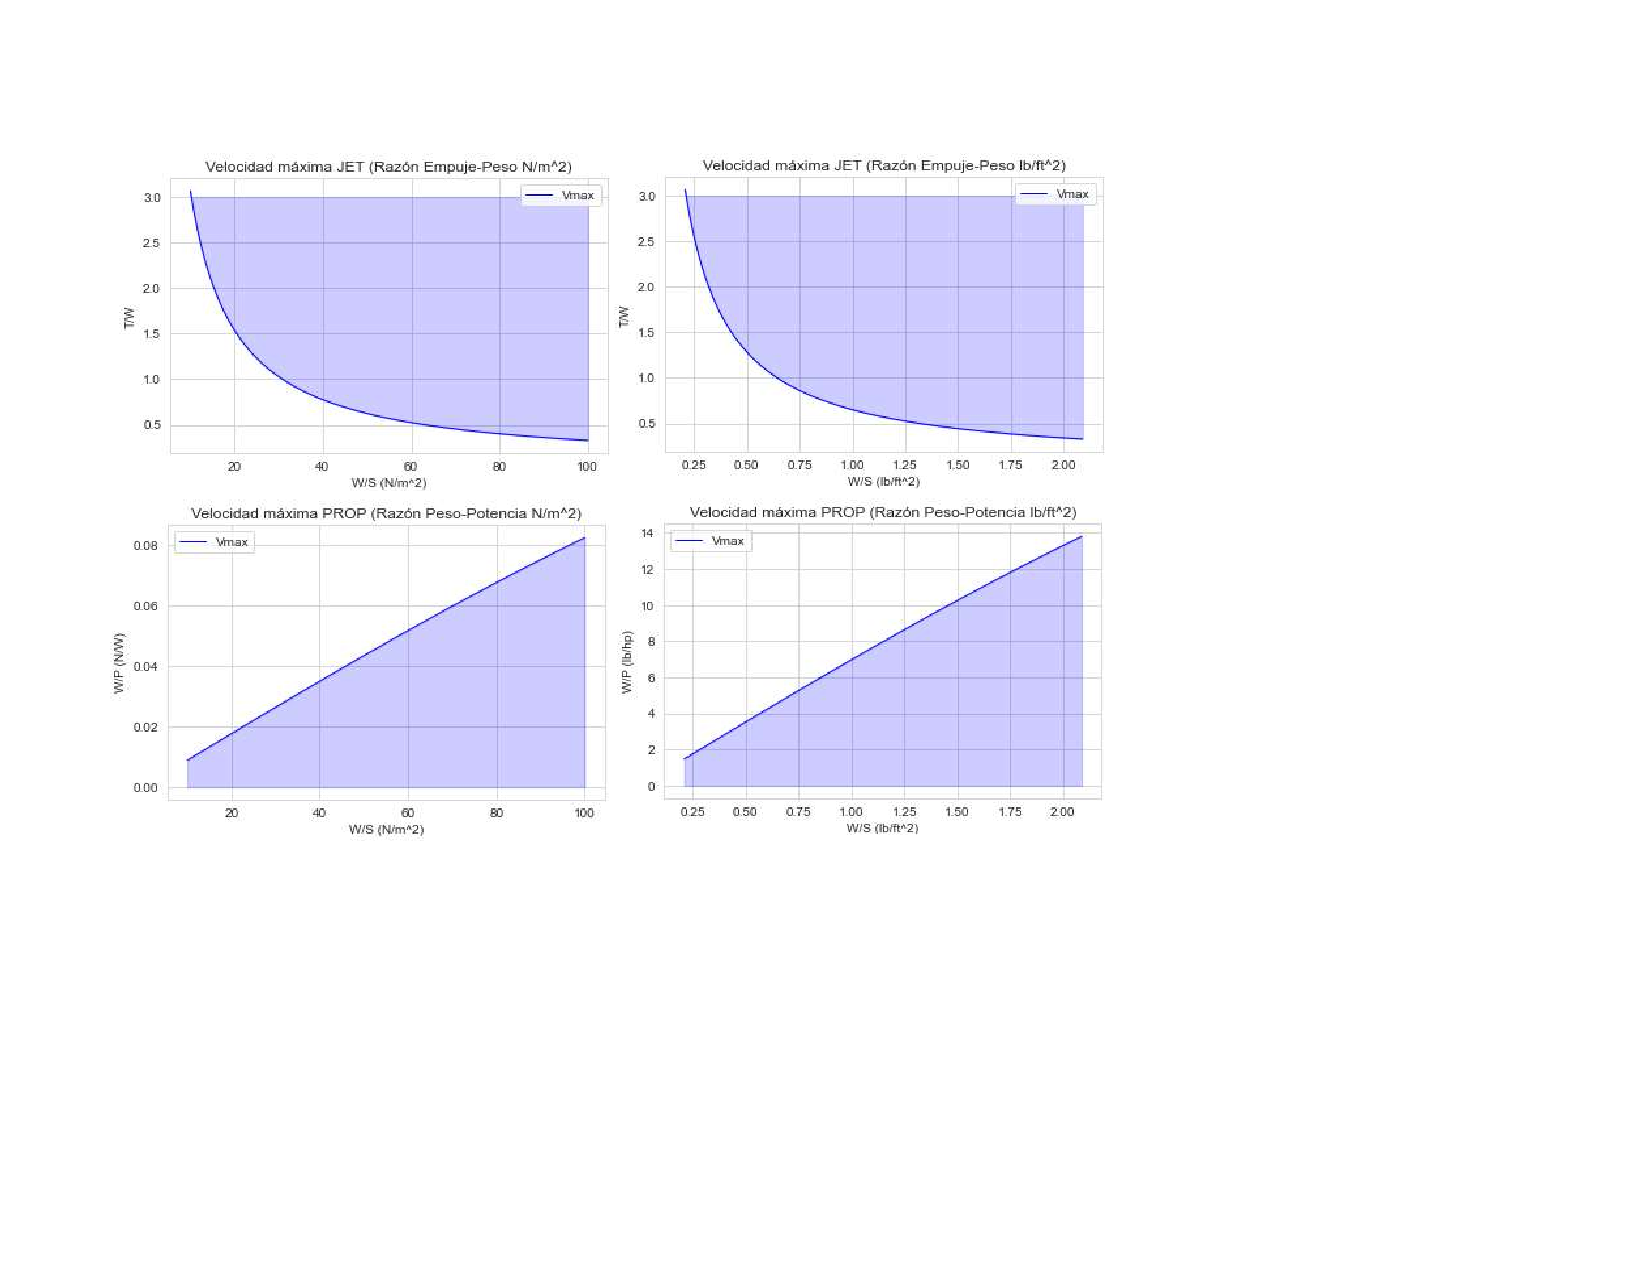
\includegraphics[scale=0.82]{Capitulo3/figs/Vmax_cropped.pdf}
\caption{Maximum speed}
\label{Vmax}
\end{figure}


\bigskip
%%%%%%%%%%%%%%%%%%%%%%%%%%%%%%%%%%%%%%%%%%%%%%%%%%%%%%%%%%%%%%%%%%%%%%%%
\textbf{Take-off runway length}\\
The take-off requirements are associated with the minimum required length of the take-off runway. 

The length of the take-off runway is defined as the point where the engines start to accelerate to where the air vehicle generates some support that makes it exceed a pre-established height. In accordance with aviation standards \cite{Sadraey2013} based on Part 25 FAR, the pre-established height to be reached by the air vehicle at the end of the runway is $35 pies$ o $10.7 m$ for passenger aircraft. However, the FAR does not establish a strict requirement for the length of the take-off runway. 

For jet or reaction engines we will use the following equation.

\begin{equation}
    (\frac{T}{W})_{S_{TO}} = \frac{\mu - (\mu + \frac{C_{D_G}}{C_{L_R}})[exp(0.6 \rho g C_{D_G} S_{TO} \frac{1}{W/S})]}{1 - exp(0.6 \rho g C_{D_G} S_{TO} \frac{1}{W/S})}
\end{equation}

Where $\mu$ is the friction coefficient of the take-off runway and $C_{D_G}$ is defined as:
\begin{equation}
    C_{D_G} = (C_{D_{TO}} - \mu C_{L_{TO}})
\end{equation}
Where the suffix $TO$ refers to the aerodynamic parameters in take-off configuration. $C_{L_R}$ is the lifting coefficient during rotation and is obtained:
\begin{equation}
    C_{L_R} = \frac{2 m g }{\rho S V_R^2}
\end{equation}
Where $V_R$ is the speed of rotation during take-off and is normally between $15-30 \%$ higher than the crash speed. If the air vehicle uses \textit{flaps} for take-off the sum of the contribution of this effector in the lifting coefficient should be considered. 

In conclusion for Jet engines, as the length of the take-off track increases, the value of the thrust-weight ratio decreases. Since any value above the minimum length established $S_{TO}$ does not meet push requirements during take-off, the part below the curve is not acceptable.   

For propeller engines we will use the following expression:
\begin{equation}
    (\frac{W}{P})_{S_{TO}} = \frac{1 - exp(0.6 \rho g C_{D_G} S_{TO} \frac{1}{W/S})}{\mu - (\mu + \frac{C_{D_G}}{C_{L_R}})[exp (0.6 \rho g C_{D_G} S_{TO} \frac{1}{W/S})]} \frac{\eta_{P}}{V_{TO}}
\end{equation}
 
The efficiency for fixed propellers at the moment of pitching have an efficiency of $0.5$ while helixes with variable pitch have an efficiency of $0.6$. As the length of the take-off track is increased, the value of the power load increases. The region above the curve is not acceptable. 

\begin{figure}[!h]
\centering
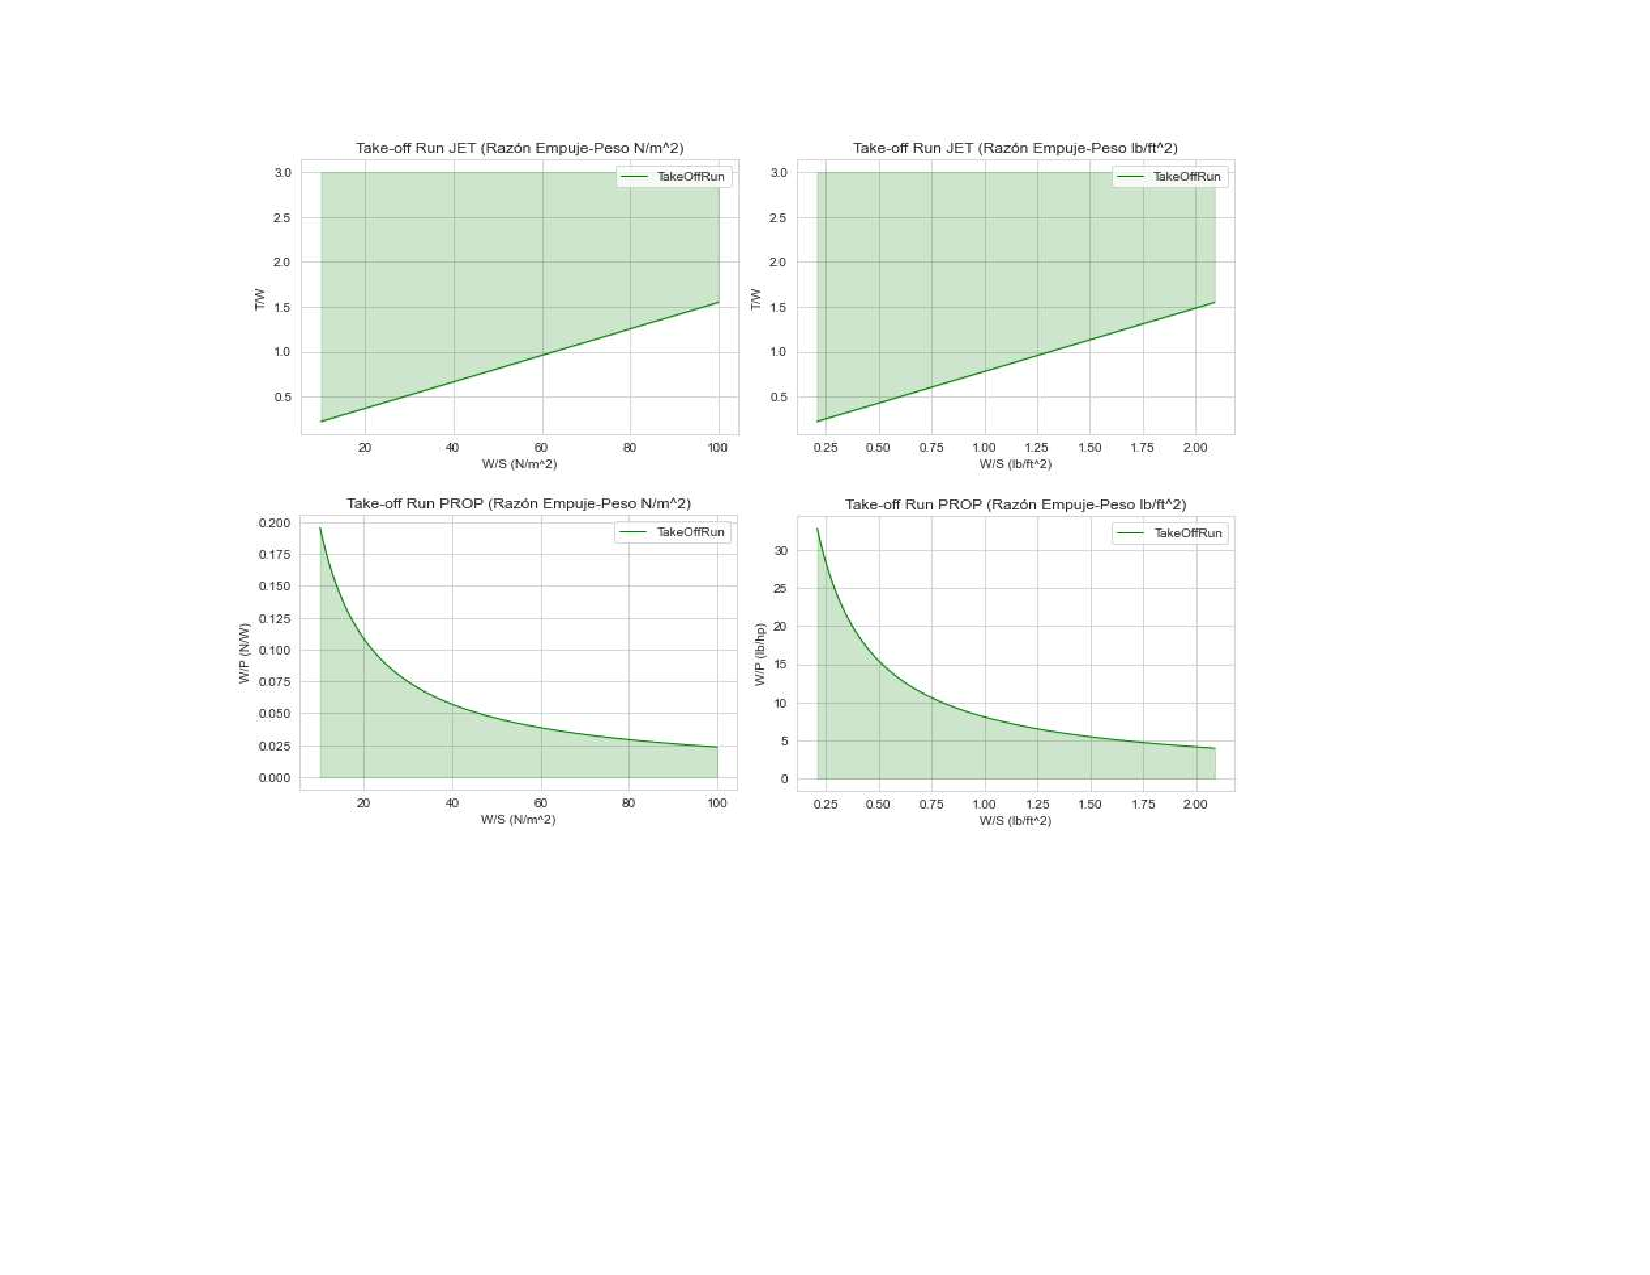
\includegraphics[scale=0.79]{Capitulo3/figs/takeoff run_cropped.pdf}
\caption{Take-off runway race}
\label{Vtakeoff}
\end{figure}

\bigskip
%%%%%%%%%%%%%%%%%%%%%%%%%%%%%%%%%%%%%%%%%%%%%%%%%%%%%%%%%%%%%%%%%%%%%%%%
\textbf{Promotional status}\\
Each type of aircraft must comply with an ascent regime. The rate of ascent is defined as the speed on the vertical axis. \textit{ROC} defines how fast the air vehicle gains altitude. 

The ROC for reaction engines is defined as the reason between the excess power and the weight of the aircraft:
\begin{equation}
    ROC = \frac{P_{avl} - P_{req}}{W} = \frac{(TV - DV)}{W}
\end{equation}
To maximize ROC we must maximize the thrust of the engines and the polar or rise-drag ratio. Then we can rewrite the above equation in:
\begin{equation}
    ROC = V[\frac{T}{W} - \frac{D}{W}] =  V[\frac{T}{W} - \frac{D}{L}] = V[\frac{T}{W} - \frac{1}{L/D}]
\end{equation}
And then:
\begin{equation}
    ROC_{max} = V_{ROC_{ma}}[\frac{T_{max}}{W}-\frac{1}{(L/D)_{max}}]
\end{equation}
Considering the minimization of the drag for the increase of polar and manipulating some terms to have a function based on the elar load we obtain:
\begin{equation}
    (\frac{T}{W})_{ROC} = \frac{ROC}{\sqrt{\frac{2}{\rho \sqrt{\frac{C_{D_0}}{K}}}(\frac{W}{S})}} + \frac{1}{(L/D)_{max}}
\end{equation}
To determine the acceptable region we must observe that side of the curve meets the requirements. As the rate of ascent increases, the value of the thrust load $(T/W)$ It also increases. Any ROC value greater than the established one meets the requirements, so the area above the curve is the acceptable region. 

for propela engines the equation is as follows:
\begin{equation}
    (\frac{W}{P})_{ROC} = \frac{1}{\frac{ROC}{\eta_{P}} + \sqrt{\frac{2}{\rho \sqrt{\frac{3 C_{D_0}}{K} (\frac{W}{S})} (\frac{1.155}{(L/D)_{max} \eta_P})}}}
\end{equation}

For this case as the value of ROC increases, the value of the thrust loading $(W/P)$ decrease. The region below the curve is acceptable, see figure \ref{ROC}. 

\begin{figure}[!h]
\centering
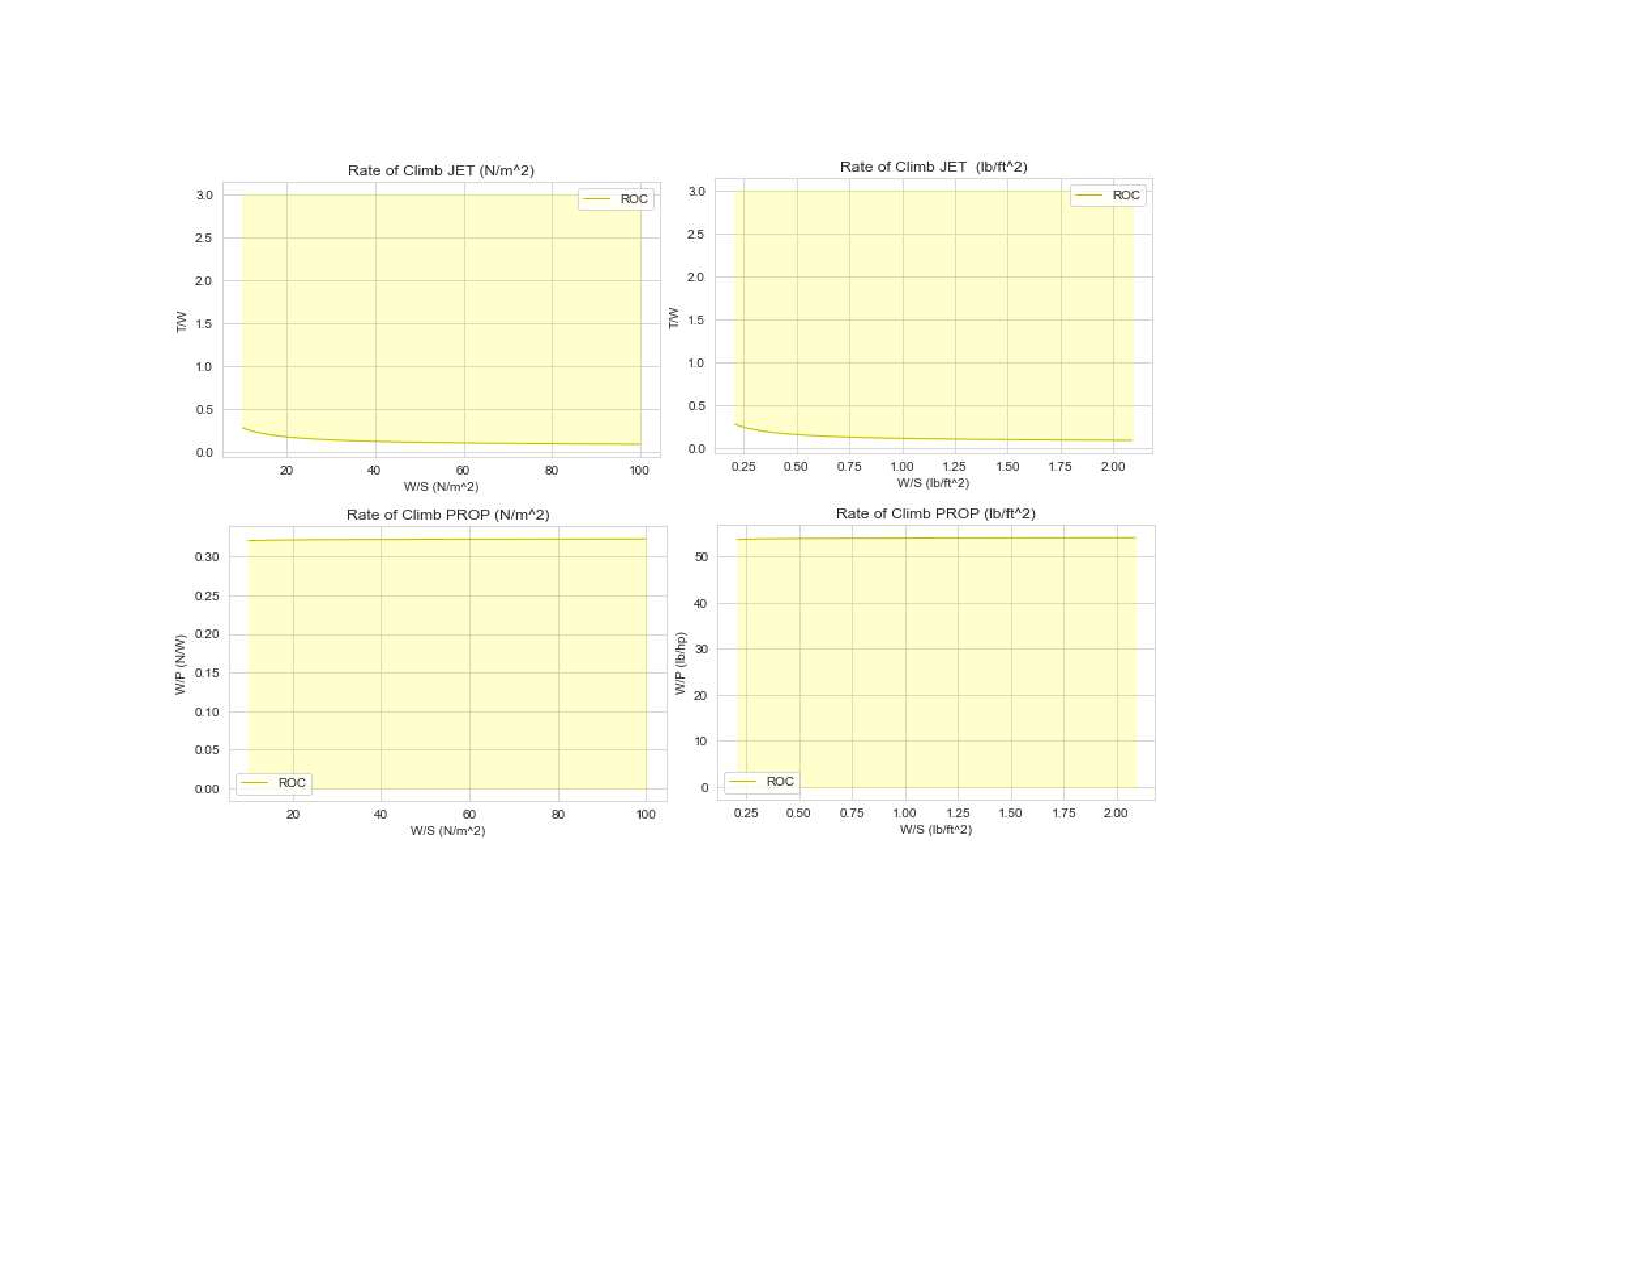
\includegraphics[scale=0.79]{Capitulo3/figs/ROC_cropped.pdf}
\caption{Promotional status}
\label{ROC}
\end{figure}

\bigskip
%%%%%%%%%%%%%%%%%%%%%%%%%%%%%%%%%%%%%%%%%%%%%%%%%%%%%%%%%%%%%%%%%%%%%%%%
\textbf{Service ceiling}\\
The \textit{techo} is defined as the maximum altitude that the air vehicle can reach having a safe straight and level flight. Another definition could be the maximum altitude to have a sustained flight according to the maximum propulsion that the engines can offer. In general, four types of roof can be defined:
\begin{itemize}
    \item Absolute roof. It is the maximum altitude that the air vehicle can maintain a safe flight straight and level. At this altitude the ascent regime is zero. 
    \item Service ceiling. It is maximum altitude that the air vehicle can reach with a regime of ascent of $100 \frac{ft}{min}, o 0.5 \frac{m}{s}$The service roof is lower than the absolute ceiling. 
    \item Cruise roof. It is the maximum altitude that the air vehicle can reach with a speed of ascent of $300 \frac{ft}{min}, o 1.5 \frac{m}{s}$.
\end{itemize}
The service and cruise roof are based on the ascent regime. For EHEKATL BWB the following are established: 
\begin{itemize}
    \item[] $ROC_{Absoluto} = 0 m/s$
    \item[] $ROC_{Servicio} = 1.25 m/s$
    \item[] $ROC_{Crucero} = 2.5 m/s$
\end{itemize}
The following equation is proposed for Jet engines:
\begin{equation}
    (\frac{T}{W})_{h_c} = \frac{ROC_c}{\sigma_C  \sqrt{\frac{2}{\rho_c \sqrt{\frac{C_{D_0}}{K} (\frac{W}{S})}}}} + \frac{1}{\sigma_C (L/D)_{max}}
\end{equation}
where $h_c$ is the maximum ceiling required for a $ROC_c$ When the aerial vehicle is in absolute roof the ROC is zero, then we can simplify the above equation with the following term:
\begin{equation}
    (\frac{T}{W})_{h_{AC}} = \frac{1}{\sigma_{AC} (L/D)_{max}}
\end{equation}
where $h_{AC}$ is the altitude of the absolute ceiling and $\sigma_{AC}$ is the density of the air in the relative according to the absolute ceiling. To determine the acceptable region we propose the following consideration: as the rate of ascent decreases the value of the thrust charge also decreases. So, any higher ROC value on the curve satisfies the requirement. 
\begin{figure}[!t]
\centering
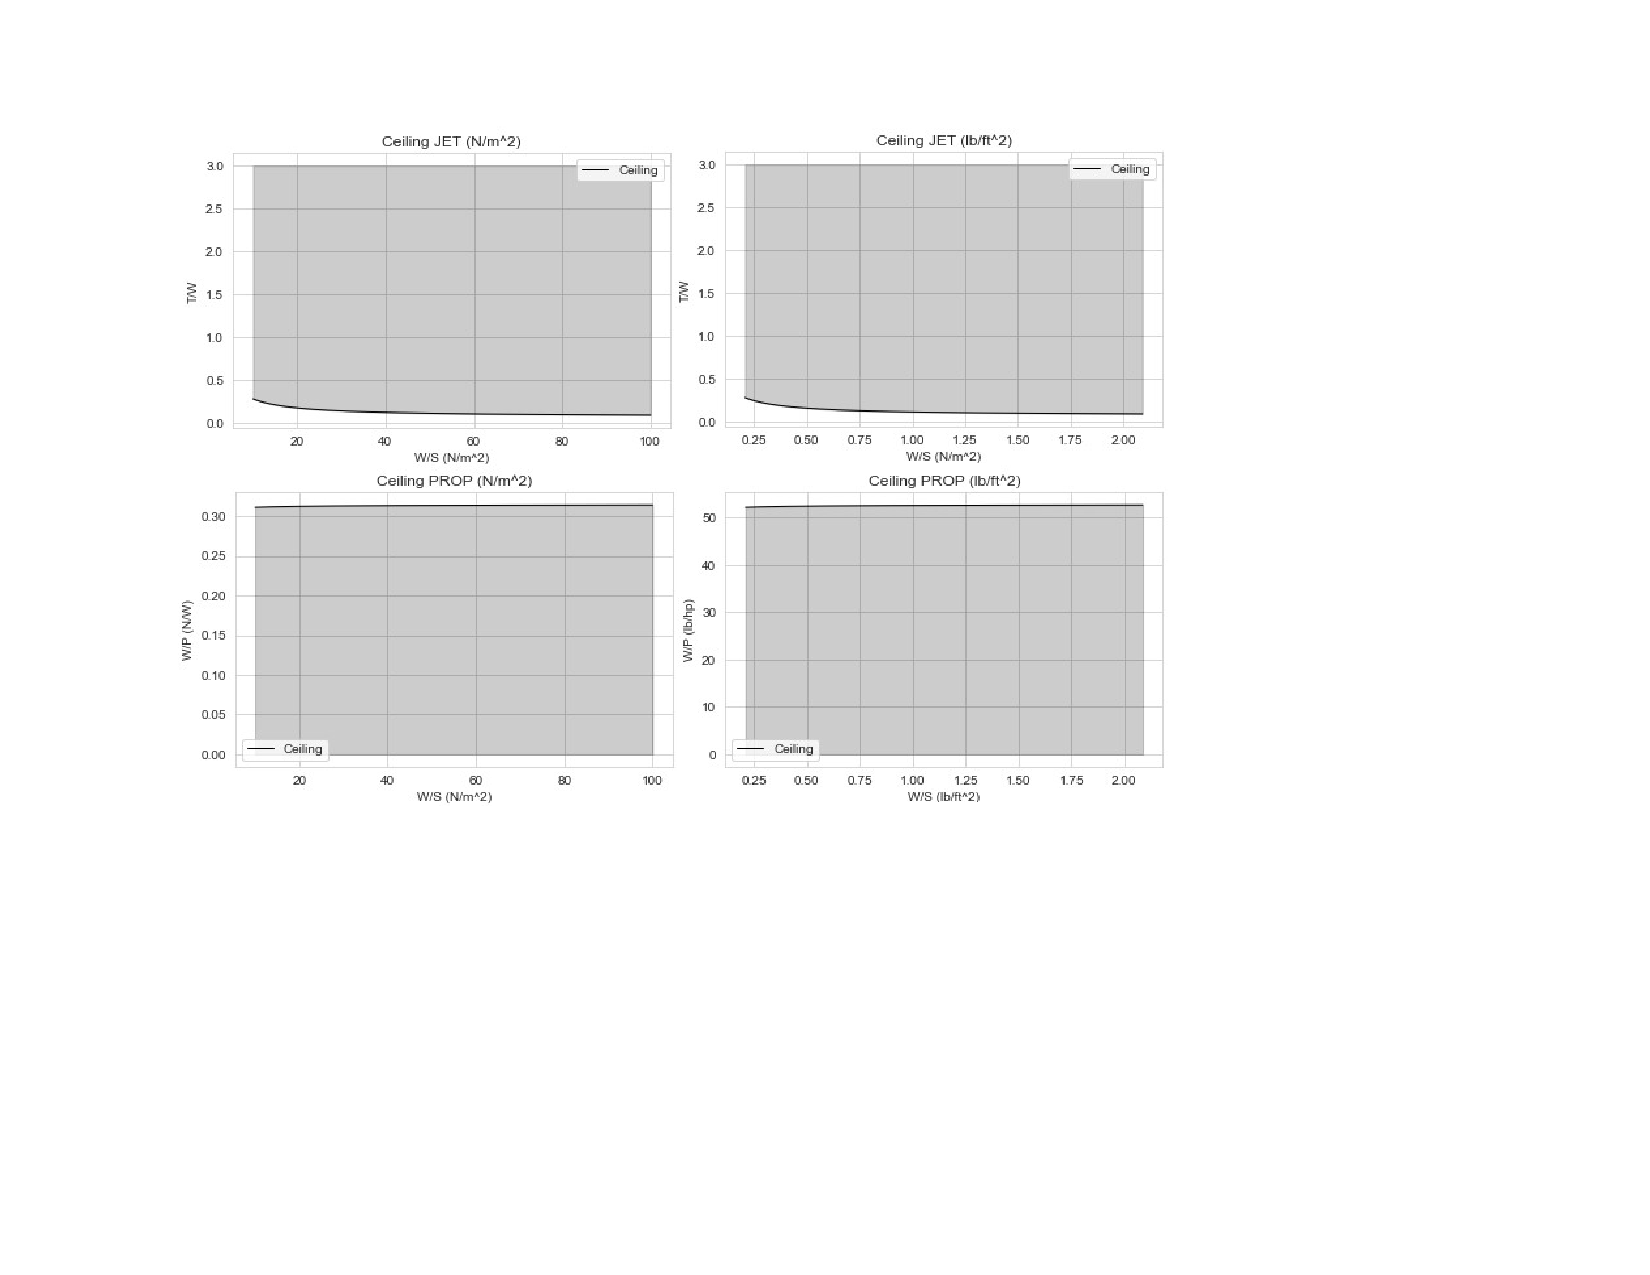
\includegraphics[scale=0.80]{Capitulo3/figs/Ceiling_cropped.pdf}
\caption{Service ceiling}
\label{Ceiling}
\end{figure}
For motors of \textbf{propellers or propellers} Let's use the next equation.
\begin{equation}
    (\frac{W}{P})_C = \frac{\sigma_C}{\frac{ROC_C}{\eta_P} + \sqrt{\frac{2}{\rho_C \sqrt{\frac{3 C_{D_0}}{K} (\frac{W}{S})} (\frac{1.155}{(L/D)_{max}\eta_P}}}}
\end{equation}
For the absolute ceiling the above expression can be simplified as follows:
\begin{equation}
    (\frac{W}{P})_{AC} = \frac{\sigma_{AC}}{\sqrt{\frac{2}{\rho_{AC} \sqrt{\frac{3 C_{D_0}}{K} (\frac{W}{S})} (\frac{1.155}{(L/D)_{max} \eta_P})}}}
\end{equation}

\bigskip
%%%%%%%%%%%%%%%%%%%%%%%%%%%%%%%%%%%%%%%%%%%%%%%%%%%%%%%%%
\textbf{Design point - \textit{Matching Plot}}\\
Now that we have the curves of the five requirements (loss speed, maximum speed, take-off track length, ascent speed and service roof) according to the power load or thrust-to-weight ratio ratio with respect to the wing load, we can integrate the five functions into the figure \ref{Punto de Diseño} to select the design point. 
%
\begin{table}[!h]
    \caption{Design Point - Matching Plot}
    \centering
    \begin{tabular}{|c|c|c|c|}
    \hline
    \multicolumn{4}{|c|}{\textbf{Motores Ductofan}}\\
    \hline
    $(\frac{T}{W})_d$ & Reason thrust-to-weight ratio & \multicolumn{2}{|c|}{$0.85$} \\
    \hline
    $(\frac{W}{S}_d$ & Wing loading &  $45 N/m^2$ & $0.9398 lb/ft^2$\\
    \hline
    \multicolumn{4}{|c|}{\textbf{Helice motors}}\\
    \hline
    $(\frac{W}{P})_d$ & Thrust loading & $0.03 N/m^2$  & $ lb/ft^2$ \\
    \hline
    $(\frac{W}{S}_d$ & Wing loading &  $50 N/m^2$ & $1.0442 lb/ft^2$\\
    \hline
    \end{tabular}
    \label{Punto de Diseño Matching Plot}
\end{table}

\begin{figure}[!h]
\centering
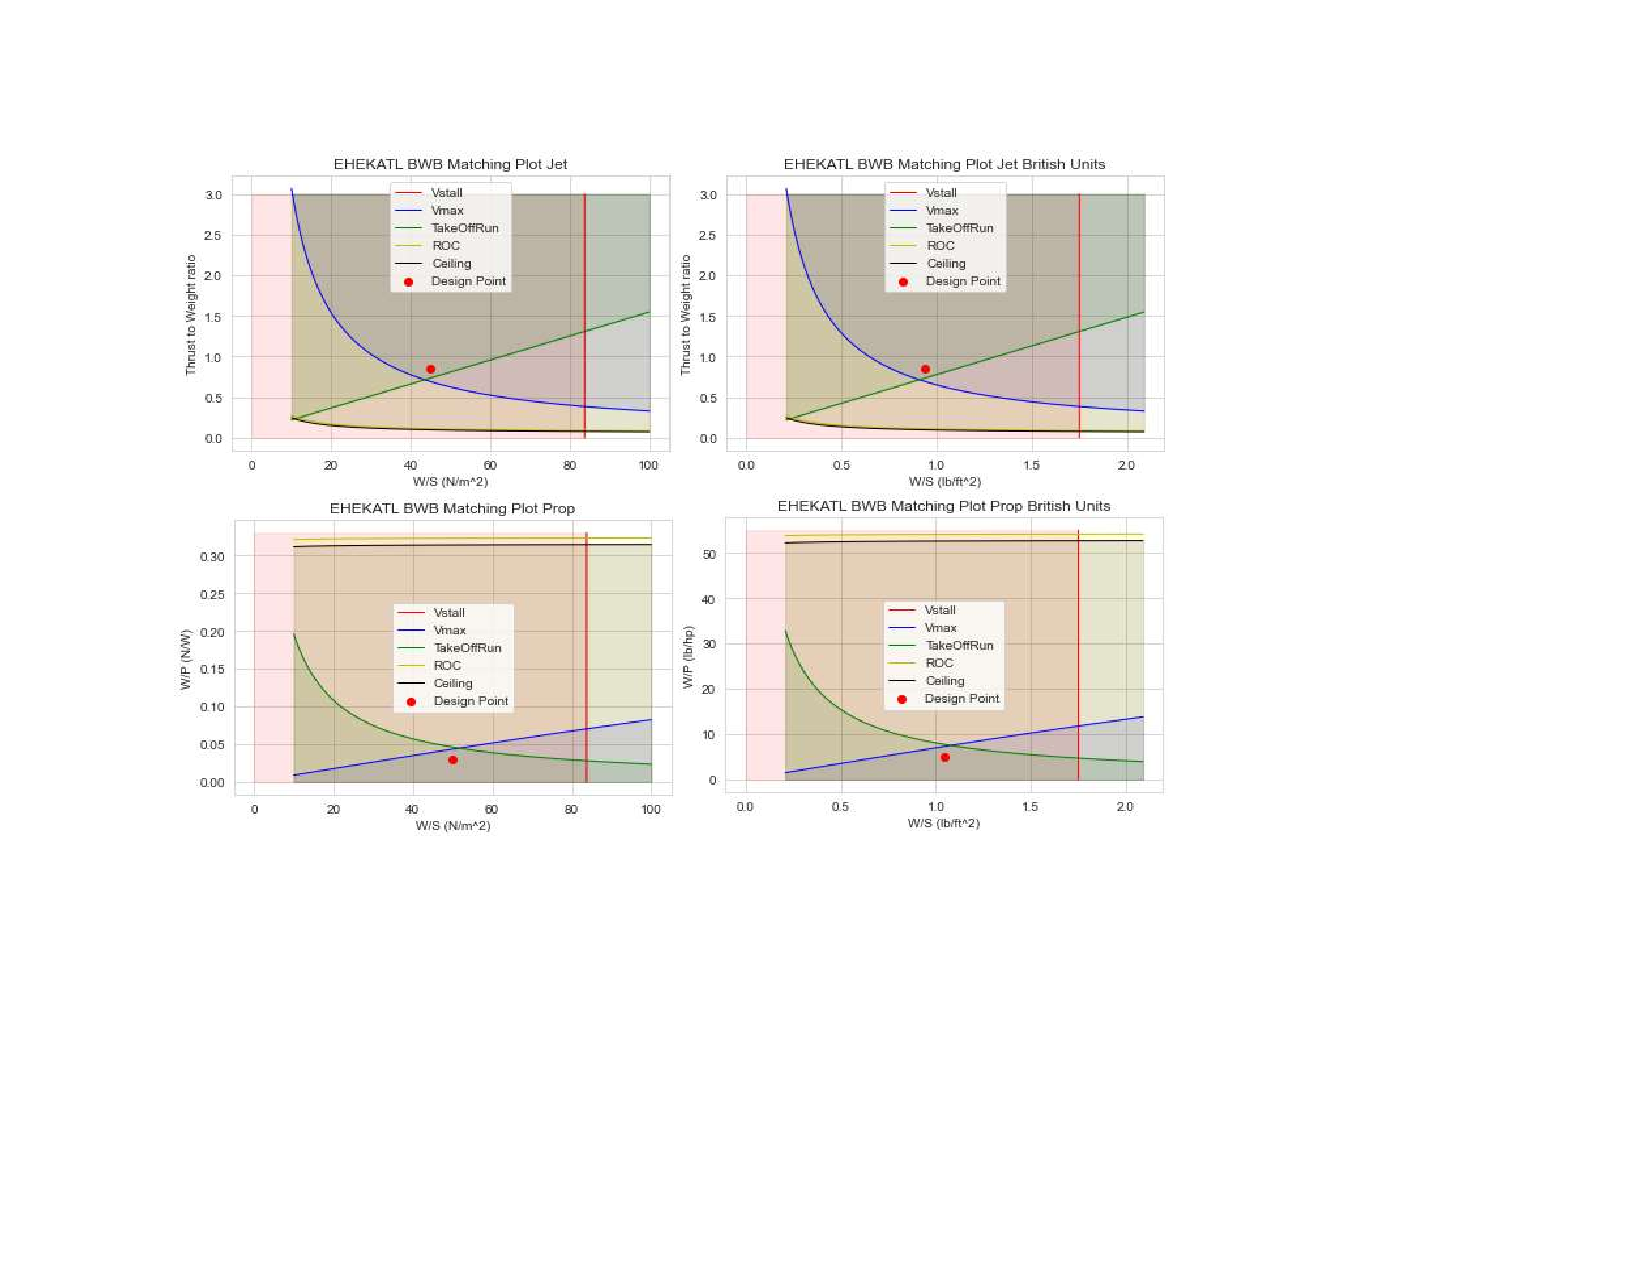
\includegraphics[scale=0.79]{Capitulo3/figs/Matching plot_cropped.pdf}
\caption{Results: Design Point with \textit{Matching Plot}}
\label{Punto de Diseño}
\end{figure}

The global acceptable region, where all requirements coincide, is the essence for the selection of the design point in \textit{Matching Plot}. 
%
According to the acceptable region shown in the figure \ref{Punto de Diseño} the design point is shown in the table \ref{Punto de Diseño Matching Plot}.

\medskip

So we can calculate the \textbf{superficie alar} and the \textbf{empuje requerido} in the following way for the \textbf{reaction engines}:

\begin{equation}
    S = \frac{W_{TO}}{(\frac{W}{S}_d)} = \frac{62 N}{45 N/m^2} = 1.375 m^2
\end{equation}

\begin{equation}
    T = W_{TO} (\frac{T}{W})_d = 62N (0.85) = 52.60N
\end{equation}

In such a way that to meet the requirements of the table \ref{Requerimientos de la misión de vuelo} EHEKATL BWB must have a minimum reference area of $1.375 m^2$ and the engines must provide a minimum thrust of $52.60N$ So that our air vehicle can take off the sidewalk. 

\medskip

Stop \textbf{propeller engines} the calculation of the \textbf{superficie alar} and the \textbf{potencia requerida} is as follows:

\begin{equation}
    S = \frac{W_{TO}}{(\frac{W}{S}_d)} = \frac{62 N}{55 N/m^2} = 1.125 m^2
\end{equation}

\begin{equation}
    P = \frac{W_{TO}}{(\frac{W}{P}_d)} = \frac{62 N}{0.033 N/W} = 1,875.06 W
\end{equation}

In such a way that to meet the requirements of the table \ref{Requerimientos de la misión de vuelo} EHEKATL BWB must have a minimum reference area of $1.125 m^2$ and the engines must provide a minimum thrust of $ 1,875.06 W$ so our air vehicle can take off. 


In the table \ref{Punto de Diseño} the final results of the wing superifice and the required power/push are shown. 

\begin{table}[!h]
    \label{superficie alar y potencia/empuje requeridos para EHEKATL BWB}
    \caption{Allar surface and power/push required}
    \centering
    \begin{tabular}{|c|c|c|c|}
    \hline
    \multicolumn{4}{|c|}{\textbf{Motores Ductofan}} \\
    \hline
      S   &  Wing area & $1.375 m^2$ & $14.80 ft^2$ \\
     T    & Minimum thrust required & $52.60N$ & $11.8249 lbf$ \\
     \hline
     \multicolumn{4}{|c|}{\textbf{Helice motors}} \\
     \hline
     S   &  Wing area & $1.125 m^2$ & $12.1093875 ft^2$ \\
     P   & Minimum Power Required & $1,875.06 W$ & $2.5125 hp$ \\
     \hline
    \end{tabular}
\end{table}

In the figure \ref{Punto de Diseño} the scheme of \textit{Matching Plot} has two optimization points within the acceptable region.
%
The first, at the intersection between the maximum speed curve and the take-off track. This point represents the minimum wing load and power/push required to achieve take-off and maintain the air vehicle. 
%
The second, at the intersection of the take-off track with the lost input speed. This point represents the maximum available wing load compared to the minimum power/push required for that load.
%
Our selection of the design point was based on the first criterion, with minimum wing load and power/push required. 
%
The aerodynamic and stability analysis presented in this chapter contemplates the results obtained from the wing surface and power required. $1.4m^2$ for EHEKATL BWB. 
%
The required power results are used for X-PLANE test simulations. 

%%%%%%%%%%%%%%%%

%%%%%%%%%%%%%%%%%%%%%%%%%%%%%%%%%%%%%%%%%%%%
\section{Proportional Integral Derivative Controller}
%%%%%%%%%%%%%%%%%%%%%%%%%%%%%%%%%%%%%%%%%%%%

Be a Derivative Integral Proportional Controller in the form:
\begin{equation}
    u(t) = K_p e(t) + K_i \int_0^t e(t) dt + k_d \dot e(t), t \geq 0 
\end{equation}  

where $K_p , K_i , K_d$ are the winning matrices for proportional, integral and derivative tuning of the tracking error $e(t)$, with $q_d(t)$ as a desired reference. 
\begin{equation}
    e(t) = q_d(t) - q(t)
\end{equation}
The component \textbf{proporcional} produces an output that is proportional to the value of the current error. \textbf{integral} adds the accumulated error in time to produce an output that is proportional to the accumulated error. \textbf{derivada} produces an output that is proportional to the rate of change of the error, \cite{Tewari2013}. 
\begin{figure}[!h]
    \centering
    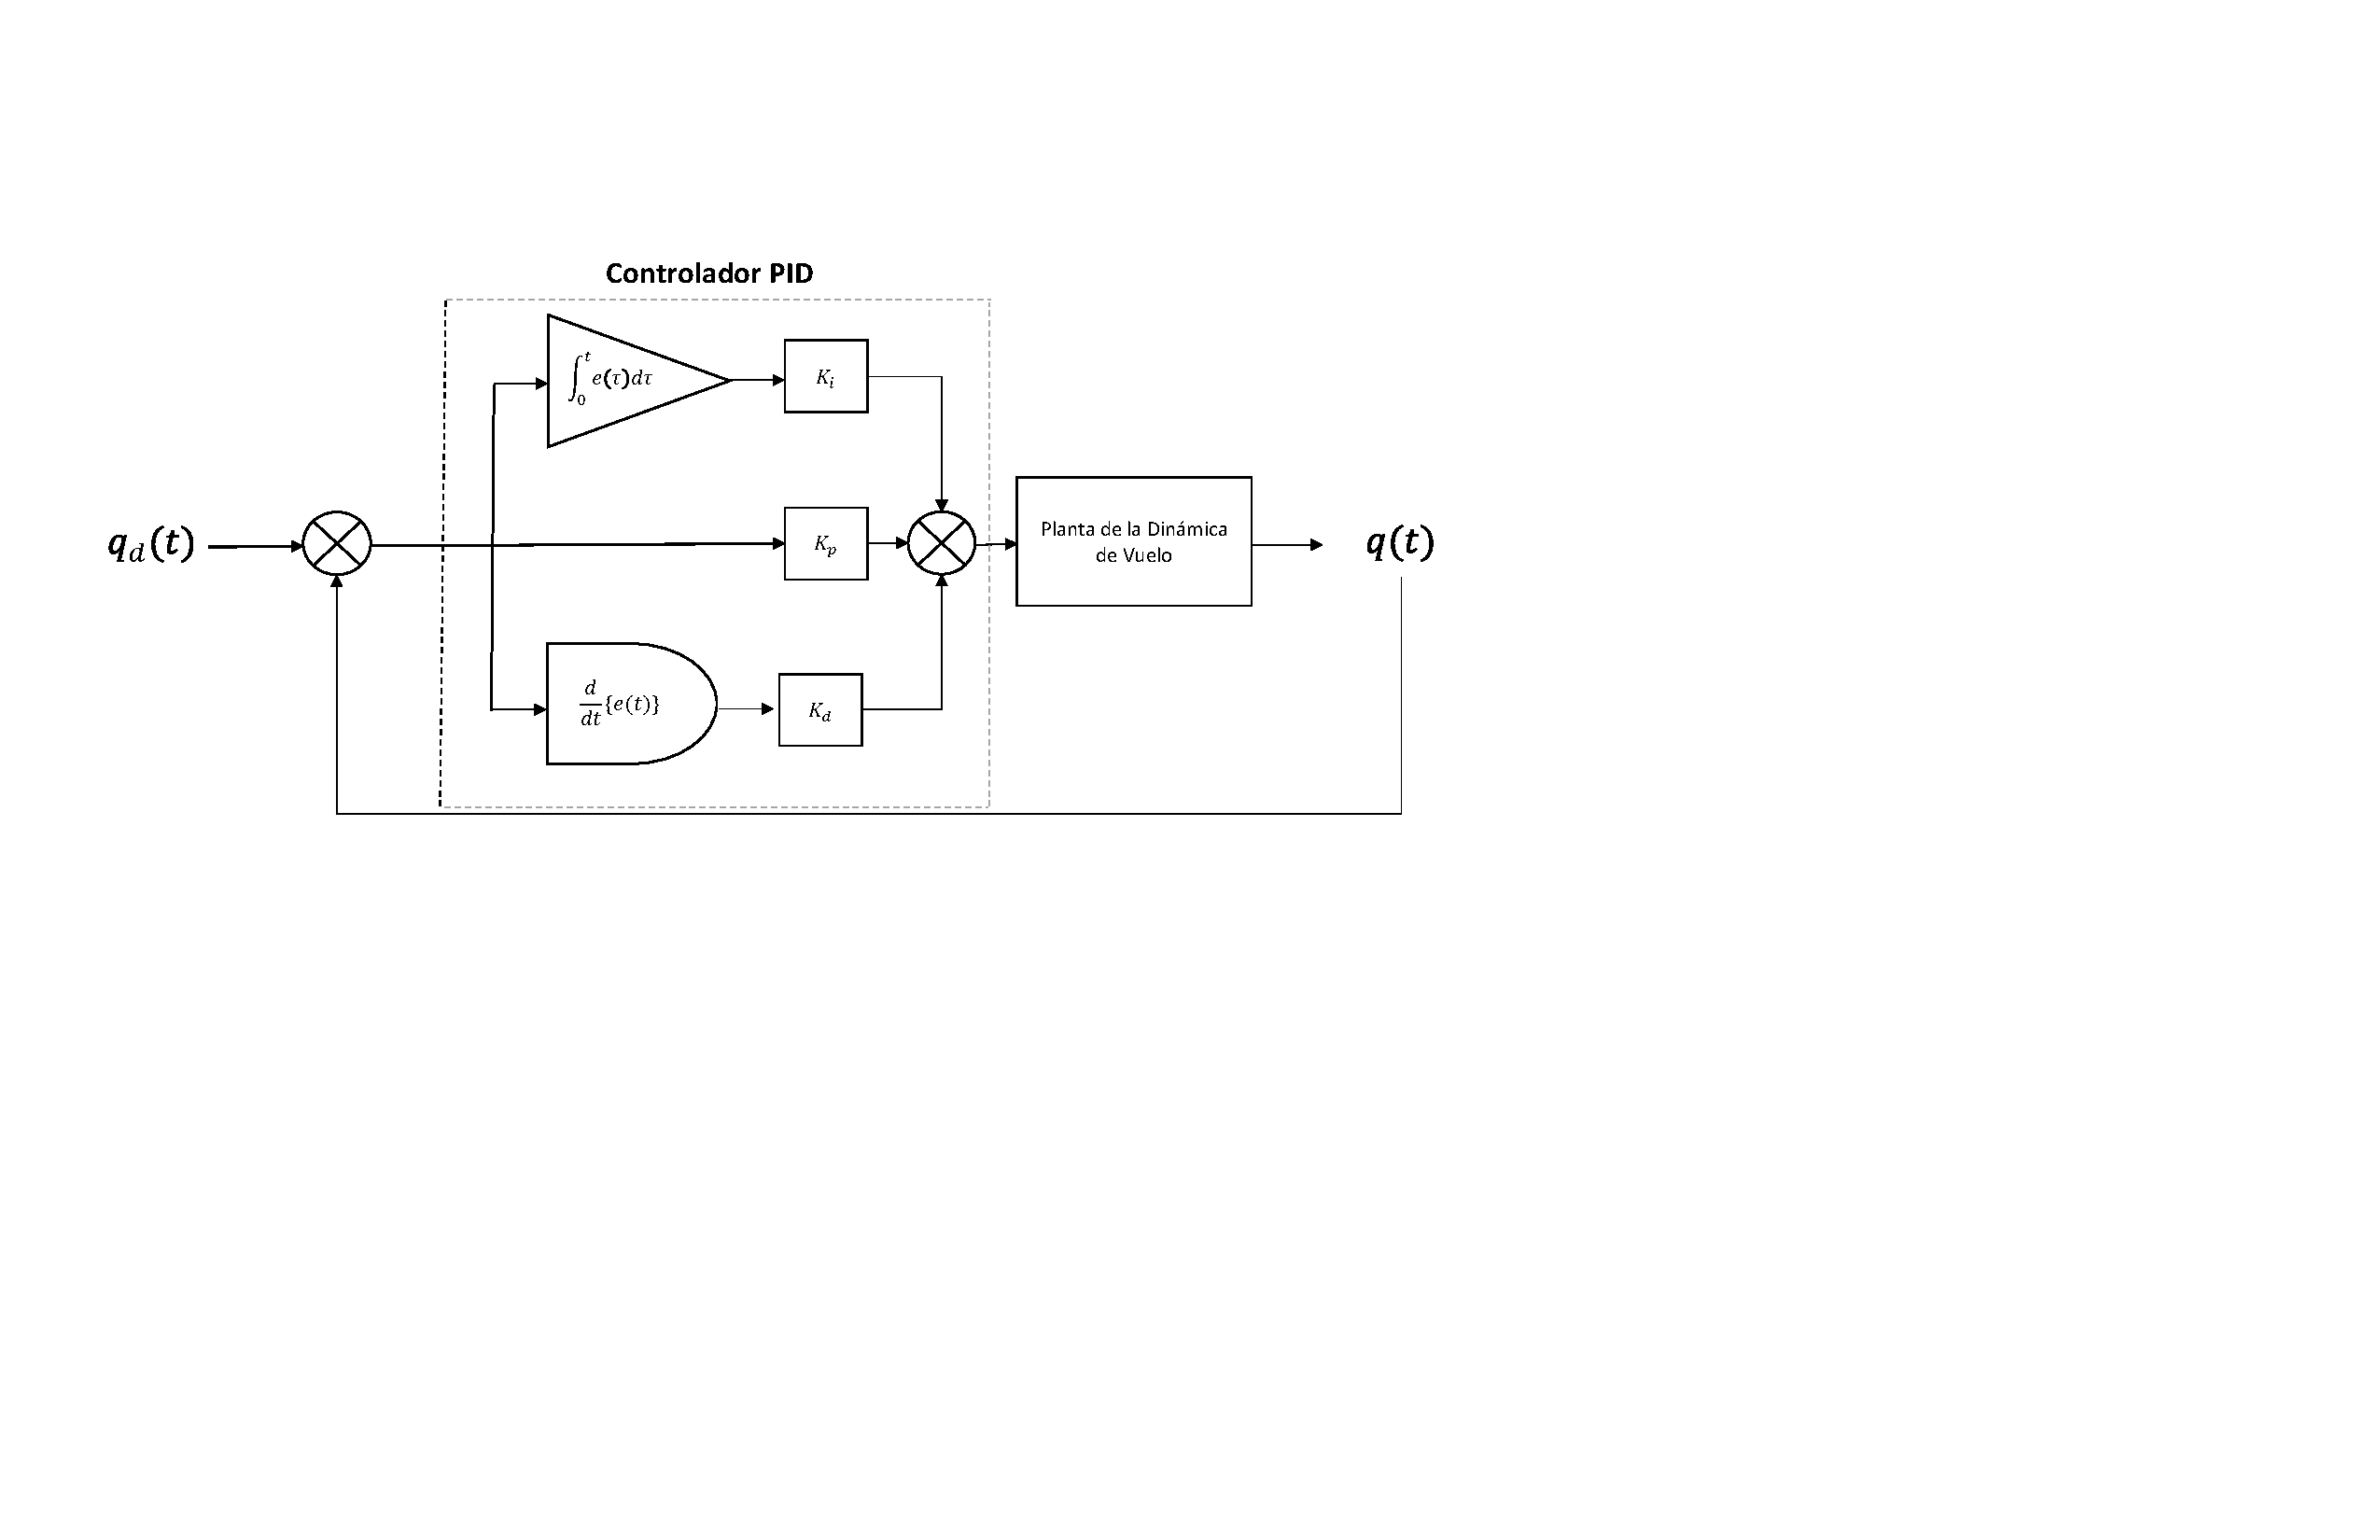
\includegraphics[scale=0.53]{Capitulo3/figs/PID new controller.pdf}
    \caption{PID controller block diagram}
    \label{fig:PID controller}
\end{figure}


The profit determination process is known as \textbf{tuning}Although the PID control was originally developed for single variable systems, its application was extended to multiple variable plants. 

The general PID driver scheme for EHEKATL BWB is shown in figure \ref{fig:PID controller}, \cite{Tewari2013}. 
%
The controller is designed as an SISO system (\textit{Single-Input, Single-Output} by its acronym in English) of single entry and single exit. For the longitudinal control are used the elevators in response to the regime of ascent \textit{ROC} or normal linear velocity $w$. For lateral control, the flaps are used in relation to the wing speed $p$. For directional control rudders are used in relation to yaw speed $r$. 

\bigskip
%%%%%%%%%%
\textbf{Simulation of PID Control for Cruise Flight}\\
The cruise flight is the phase of the flight mission with the longest duration, and is characterized by being a flight where the altitude and speed are constant and the variation in the angle of attack is small, in addition, it is a wing-level flight where the angular speed of rolling and yawing are considered non-significant and we can be negligent with the lateral and directional dynamics. 
%
The main function of the PID flight controller during EHEKATL BWB cruise flight is to compensate for disturbances that might occur during the cruise flight to maintain the nodding attitude and a certain angle of attack, in addition to governing the ascent regime to achieve the desired altitude. 

The simulation will be done through a representation in state spaces of the linear longitudinal model of EHEKATL BWB seen in \ref{lineal longitudinal cuerpo}-\ref{lineal longitudinal cuerpo 1} considering a \textbf{continuous system invariant over time}, see equation \ref{longitudinal lineal EHEKATL BWB}.
\begin{equation}
\label{longitudinal lineal EHEKATL BWB}
    \begin{bmatrix}
        \dot u \\
        \dot w \\
        \dot q \\
        \dot \theta
    \end{bmatrix}
    =
    \begin{bmatrix}
    -0.0406476 & 0.651139 & 0 & -9.81 \\
    -1.5108 & -4.21972 & 10.9907 & 0 \\
    -7.04976e-08 & -2.99525 & -4.33042 & 0 \\
    0 & 0 & 1 & 0 \\
    \end{bmatrix}
    \begin{bmatrix}
        u \\
        w \\
        q \\
        \theta
    \end{bmatrix}
    +
    \begin{bmatrix}
    0.4311 \\
    -13.2133 \\
    -27.35 \\
    0\\
    \end{bmatrix}
    \delta_e
\end{equation}

Dimensional aerodynamic parameters of the equation \ref{longitudinal lineal EHEKATL BWB} were obtained through a stability analysis with XFLR5, where a mass was considered $m$ of $6.31kg$ and stability analysis throws a moment of inertia $I_y$ of $0.8856 kgm^2$ at a speed of $13.23m/s$ with an angle of attack $12.82^{\circ}$. The tracking error is defined as the reason for the desired altitude $w_d (t)$ minus the actual altitude ratio of EHEKATL BWB $ w(t)$. 
\begin{equation}
    e (t) = w_d (t) - w(t)
\end{equation}

The tuning of the PID driver gains is shown in the Table \ref{Ganancias del Controlador PID Longitudinal}. 
\begin{figure}[!t]
    \centering
    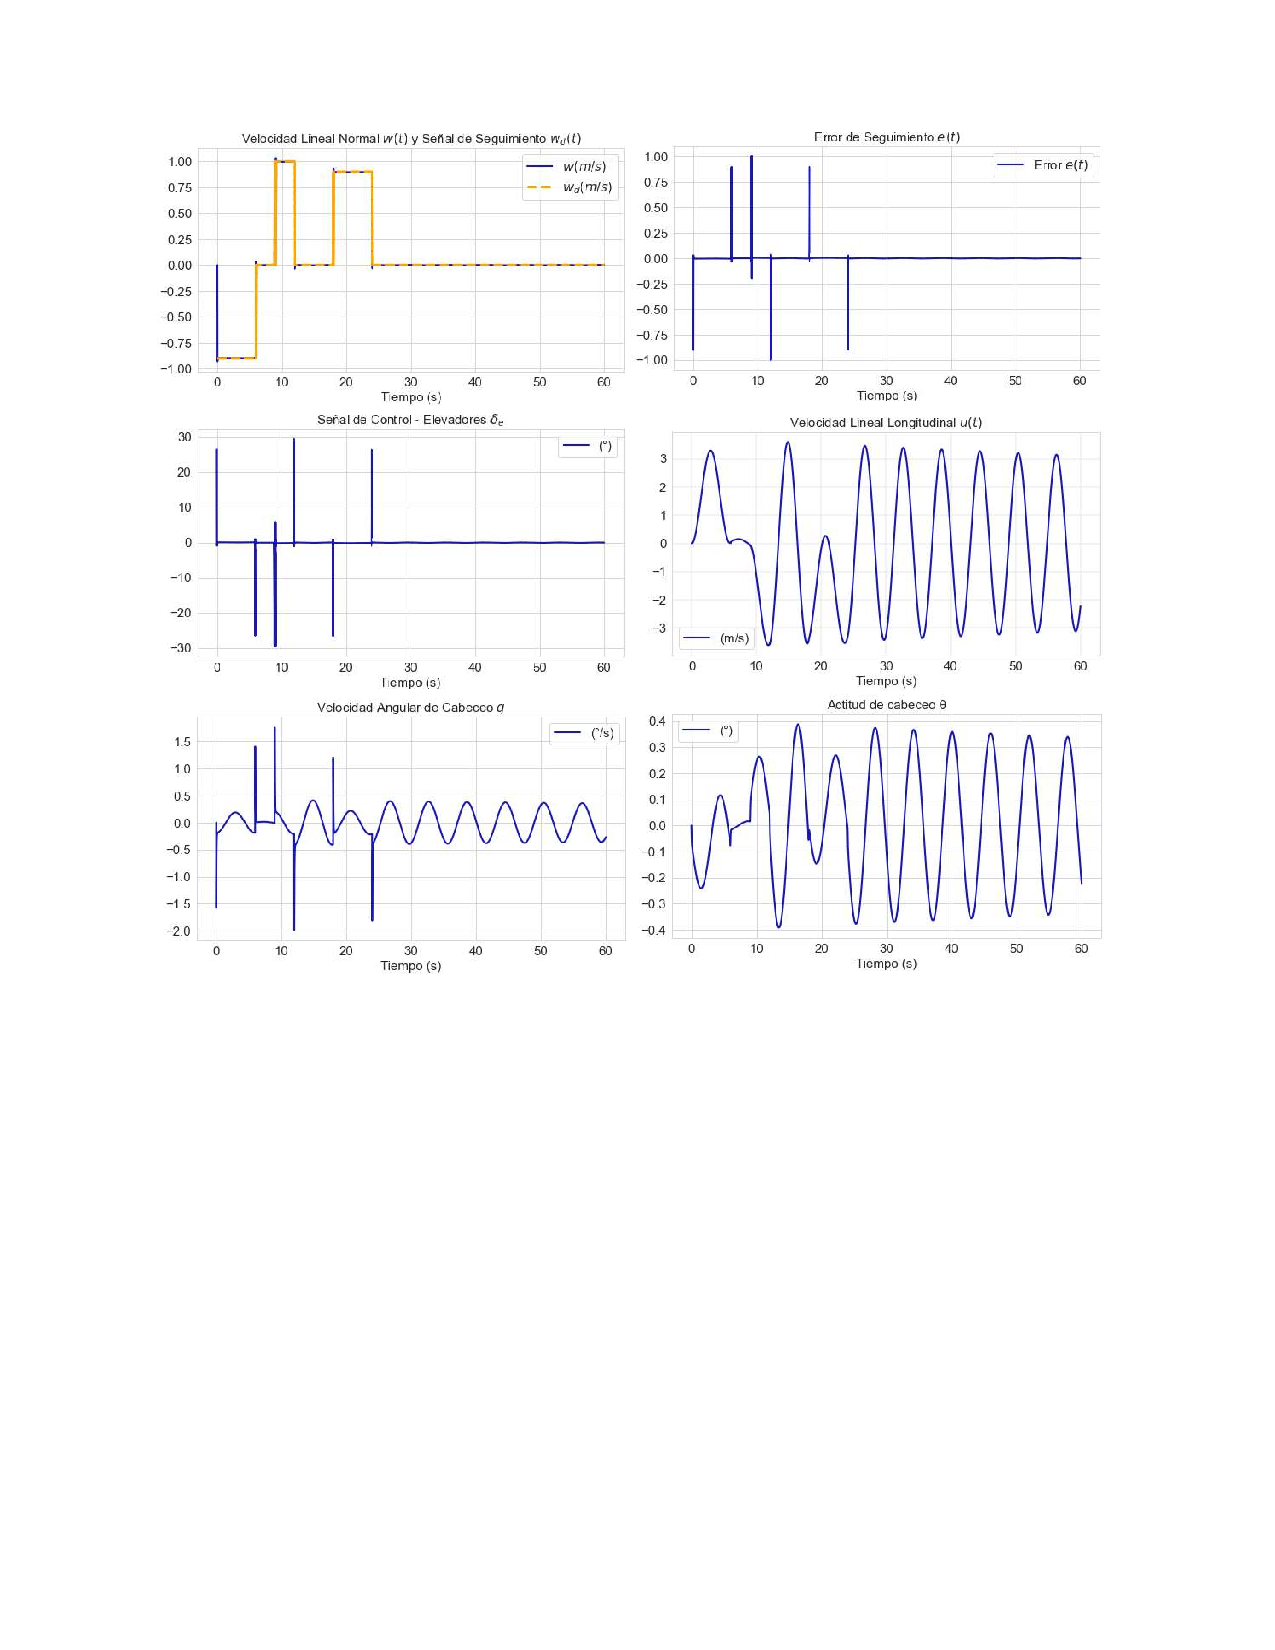
\includegraphics[scale=0.84]{Capitulo3/figs/Simulacion PID crucero_cropped.pdf}
    \caption{Flight Simulation Cruise with PID Controller}
    \label{Simulación de Vuelo Crucero con Controlador PID}
\end{figure}
\begin{table}[!h]
    \centering
    \begin{tabular}{|c|c|}
    \hline
    \multicolumn{2}{|c|}{Longitudinal PID Controller Gains}\\
    \hline
     Proportional $k_p$ & $-25.150989512082$ \\
     Integral $k_i$ & $-715.814283072008$\\
     Derivative $k_d$ & $0.0334264493487736$\\
     \hline
    \end{tabular}
    \caption{Longitudinal PID Controller Gains}
    \label{Ganancias del Controlador PID Longitudinal}
\end{table}

\textbf{Results discussion.} Figure \ref{Simulación de Vuelo Crucero con Controlador PID} shows the results of the PID controller for the longitudinal dynamics of EHEKATL BWB. According to the oscillatory movement in $q(t)$,$\theta(t)$ and $u(t)$ a fugoid longitudinal mode is observed with free controls. The follow-up signal is proposed $w_d$, see graph a). $w_d$ It aims to imitate an initial disturbance that forces the aircraft to rise slightly (negative sign) its altitude for six seconds. It regains its constant altitude briefly when a second disturbance manages to descend it for three seconds. The aircraft recovers for an instant the altitude to descend again by a third and final disturbance, to finally maintain at constant altitude. 
%
In graph b) the behavior of the tracking error over time is shown. the tracking error $e(t)$ grows as much as the follow-up signal $w_d (t)$ This means that the PID controller is performing an excellent follow-up task according to the gains proposed in \ref{Ganancias del Controlador PID Longitudinal}. 
%
Figure (c) shows the response of the elevators $\delta_e$ to meet the desired path of $w_d$. The response of the elevators is very fast and is in the deflection range of $-30^\circ /+30 ^\circ$. 
%
Graph d) shows longitudinal linear velocity $u(t)$. Here, the zero nominal value does not represent a state at rest but a uniform or constant speed of $13.23m/s$. So, the increase or decrease of the speed $u(t)$ is an addition or subtraction to this constant speed. It is observed that the speed maintains an oscillatory movement due to which EHEKALTL BWB maintains a slight tilt swing with the control inputs (lifts) free. $w_d$ demand a change in the trajectory generated by the elevators $\delta_e$ A change response is perceived in the oscillatory movement of $u(t)$. When $w_d$ is kept at zero, $u(t)$ continues with oscillatory movement with fixed elevators. 
%
Graph (e) shows the angular pitching speed $q$. It is noted that it responds in the same way as the follow-up signal $w_d$. Maintains a less oscillatory movement than $-0.5/0.5$ degrees. 
%
Finally, graph f) shows the pitching attitude $\theta$. The response of $\theta$ is in the same sense as $w_d$. Keeps a smooth oscillatory movement between $-0.4 / 0.4$ degrees. 

\medskip

%%%%%%%%%%%%%%%%%%%%%%%%%%%%%%%%%%%%%%%%%%%%%%%%%%%%%%
\textbf{PID Control Simulation for Lateral Spin}\\
When an aircraft rotates to one side or the other, it is due to the difference in lift generated at the end of the wing due to the deflection of the wings. As mentioned in the dynamic model, the deflection of the pair of wings in the opposite direction generates a lateral twist. Although the lateral dynamics use both the wings and the rudders, the main contribution to a twist is mostly from the wings (around a $80\%$ Depending on the type of aircraft and the conditions of flight). The rudders are usually used to adjust the direction or direction of the nose and get a smooth lateral movement. For the application of the PID control in EHEKATL BWB we will use the tracking signal $p_d$ for the control of the angle speed of rolling $p$. This application aims to control the lateral rotation speed, and integrating to obtain the translation position on the axis \textit{and} The objective of the EHEKATL BWB lateral PID controller is to maintain sustained rotations at different speeds and return to the wing level flight. The aircraft is assumed at a constant speed of $13.23 m/s$ to make a sustained turn. The equation \ref{PID lateral EHEKATL BWB} shows the lateral dynamics of EHEKATL BWB representing state space for the simulation of the linear system invariant over time. 
\begin{equation}
\label{PID lateral EHEKATL BWB}
    \begin{bmatrix}
        \dot v \\
        \dot p \\
        \dot r \\
        \dot \phi
    \end{bmatrix}
    =
    \begin{bmatrix}
    -0.440144 & -0.263171 & -16.0681 & 9.81 \\
    -8.22254 & -22.4261 & 8.34045 & 0 \\
    2.0262 & 1.4176 &-1.72499 & 0 \\
    0 & 1 & 0 & 0 \\
    \end{bmatrix}
    \begin{bmatrix}
        v \\
        p \\
        r \\
        \phi
    \end{bmatrix}
    +
    \begin{bmatrix}
    2.882972 \\
    500.764 \\
    -18.97689 \\
    0\\
    \end{bmatrix}
    \delta_a
\end{equation}

The tracking error is defined as the desired signal of the rolling regimen $p_d(t)$ minus the actual signal of the EHEKATL BWB wing regime $p(t)$. 
\begin{equation}
    e(t) = p_d (t) - p(t)
\end{equation}
\begin{figure}[!h]
    \centering
    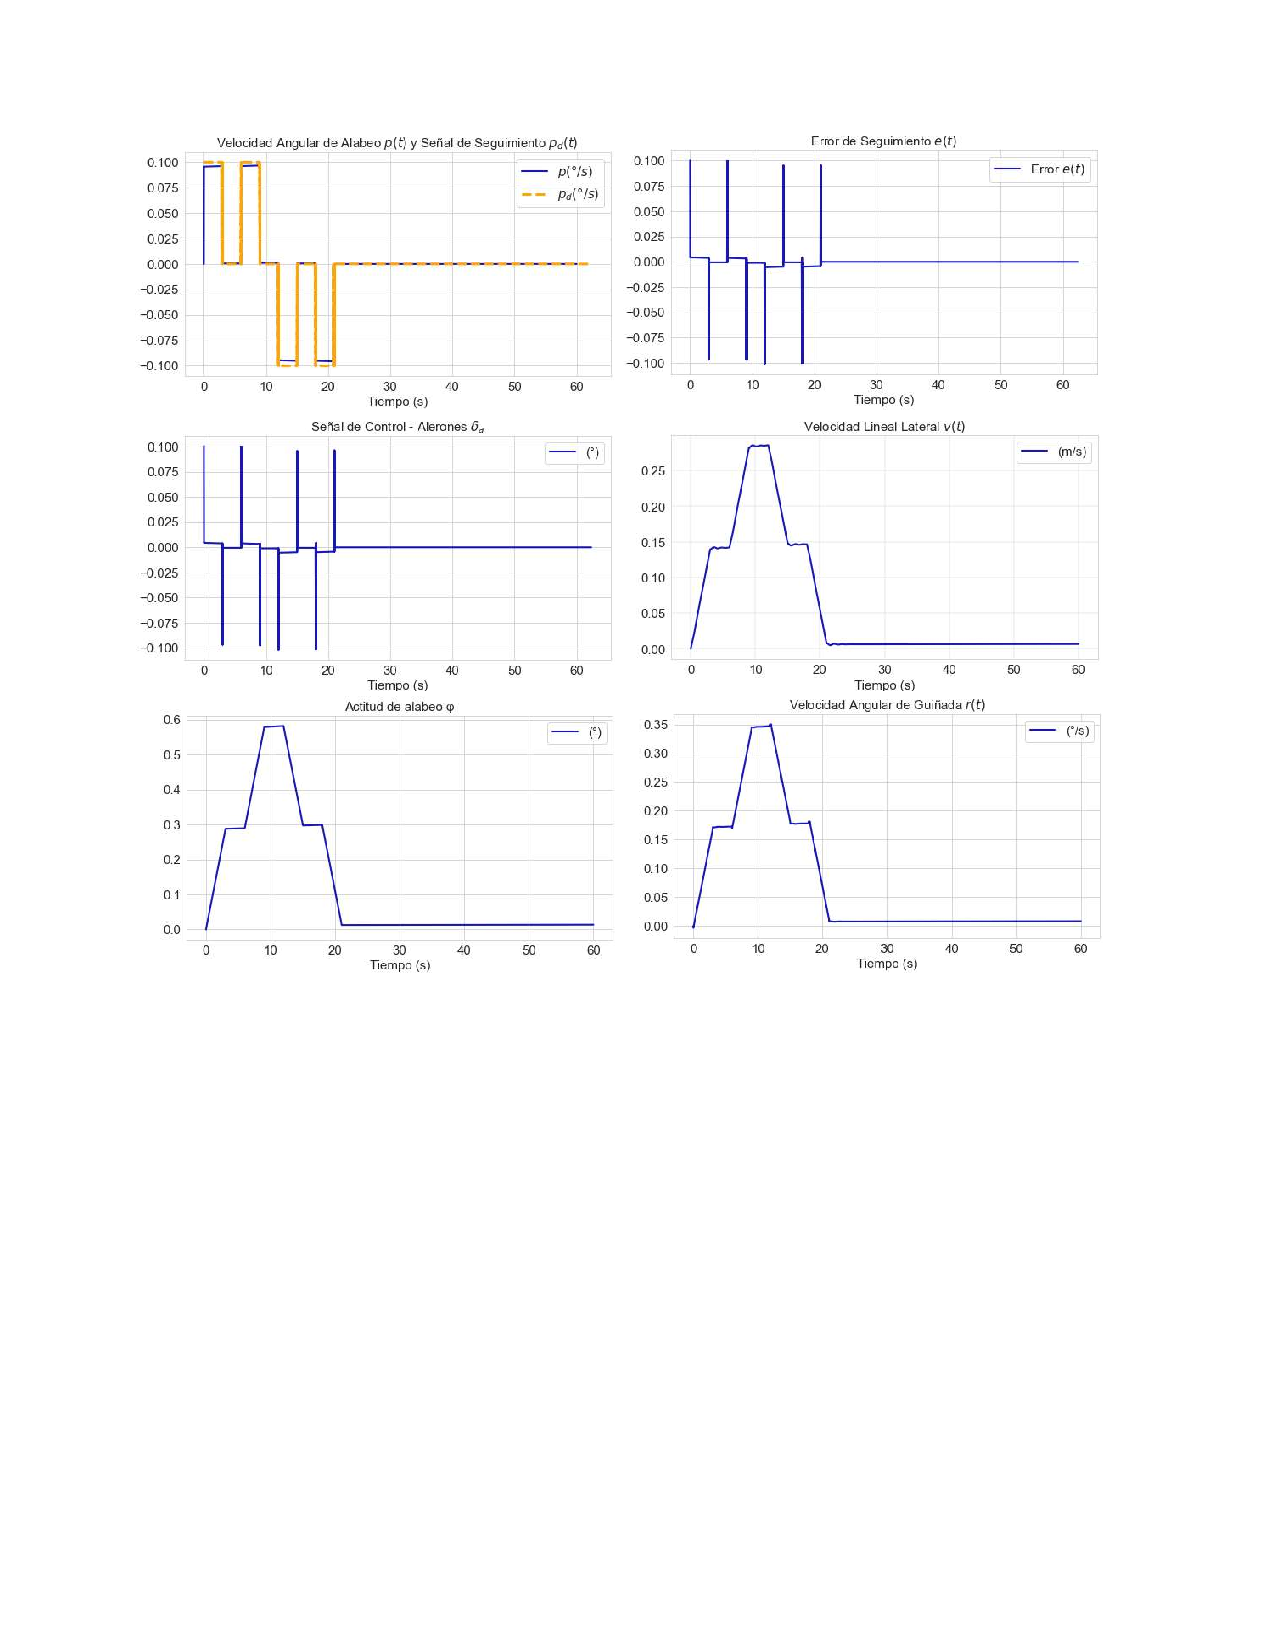
\includegraphics[scale=0.82]{Capitulo3/figs/Simulacion PID lateral_cropped.pdf}
    \caption{Lateral Spin Simulation with PID Controller}
    \label{Simulación de Giro Lateral con Controlador PID}
\end{figure}

Side PID driver gains are shown in the Table \ref{Ganancias del Controlador PID Lateral}.
\begin{table}[!h]
    \centering
    \begin{tabular}{|c|c|}
    \hline
    \multicolumn{2}{|c|}{PID Controller Gains}\\
    \hline
     Proportional $k_p$ & $0.0393742116172623$ \\
     Integral $k_i$ & $1.39969270141192$\\
     Derivative $k_d$ & $0$\\
     \hline
    \end{tabular}
    \caption{PID Lateral Driver Gains}
    \label{Ganancias del Controlador PID Lateral}
\end{table}

\textbf{Discussion of the Results.} In the Figure \ref{Simulación de Giro Lateral con Controlador PID} the results of the EHEKATL BWB sustained rotation simulation are observed.
%
According to graph (a) the tracking signal $p_d$ determines the speed of rotation (reason or speed). Although the gains of the PID side controller in the Table \ref{Ganancias del Controlador PID Lateral}  make the sign of the reason for roll $p$ fast approach to follow-up signal $p_d$He can't reach it, even if he stays very close. $p_d$ It is intended to operate a right turn (positive value) in a speed that increases to a ratio of 0.1 degrees per second during the first seconds. It is maintained in this sustained turn to increase again the wing speed at the same rate of 0.1 degrees per second before the first ten seconds. It is maintained for an instant after decreasing the speed of rotation achieved with an equal but opposite magnitude (negative values) respecting the same intervals as the first two passing signals. This consideration causes EHEKATL BWB to regain flight at wing level shortly after the second wind. 
%
Chart b) shows the tracking error $e(t)$. Here it is noted that since the actual sign of rolling regime $p(t)$ does not reach the follow-up signal $p_d(t)$ the follow-up error $e(t)$ does not reach zero after passing signals. However, only a straight line or peaks are distinguished in $e(t)$ given the quick response of the controller. 
%
Chart (c) shows the control signal of the ailerons $\delta_a$. The response is fast and within the deflection range of $-0.1 / 0.1$ degrees. 
%
Chart d) shows the linear lateral velocity $v(t)$. This velocity is the one that determines the lateral linear position change. According to the first step signal $p_d$, $v(t)$ achieves a reason for displacement of $0.14m/s$. With the second step sign achieves a reason for $0.28m/s$. The next sign, already with negative sign, descends to $v(t)$ back to a reason for  $0.14m/s$ to finally with the last pass signal regain the flight at wing level with $v(t)$ equal to zero. 
%
Graph (e) shows the attitude of roll $\phi(t)$. with the first sign of passage is achieved an attitude of roll towards the right of almost $0.3 ^\circ$. With the second sign of passage the attitude of the highest roll of little less than $0.6 ^\circ$. 
%
Finally, graph f) shows the yaw speed $r(t)$ with respect to the axle $z$. In the first step sign it is possible to maintain a $r(t)$ of $17 ^\circ/s$ for the second step sign to maintain a $r(t)$ maximum of $0.34 ^\circ/s$.


\bigskip

\textbf{Simulation of PID Control for Run or Direction}\\
The course refers to the direction in which the aircraft's nose is pointing. It's an orientation that normally takes the axis. $x$ With a northerly direction as an initial reference. A tyawled stable aircraft maintains a fixed direction without the pilot’s intervention. Maintaining the course is essential for tracking the flight path, for example. For the directional PID controller of EHEKATL BWB we will use the tracking signal $r_d$ for the control of the yaw ratio $r$. The tracking error is defined as the desired signal  $r_d(t)$ minus the yaw speed of EHEKATL BWB $r(t)$. 
\begin{equation}
    e(t) = r_d (t) - r(t)
\end{equation}
The same conditions are assumed at a constant speed of $13.23 m/s$ to perform the maneuvers of yaw, direction or direction. \ref{direcciooal lineal EHEKATL BWB} The directional dynamics of EHEKATL BWB are shown in state space representation for the simulations of the linear system invariant over time. 
\begin{equation}
\label{direcciooal lineal EHEKATL BWB}
    \begin{bmatrix}
        \dot v \\
        \dot p \\
        \dot r \\
        \dot \phi
    \end{bmatrix}
    =
    \begin{bmatrix}
    -0.440144 & -0.263171 & -16.0681 & 9.81 \\
    -8.22254 & -22.4261 & 8.34045 & 0 \\
    2.0262 & 1.4176 &-1.72499 & 0 \\
    0 & 1 & 0 & 0 \\
    \end{bmatrix}
    \begin{bmatrix}
        v \\
        p \\
        r \\
        \phi
    \end{bmatrix}
    +
    \begin{bmatrix}
    4.206642e-13 \\
    -7.63414e-11 \\
    1.48159e-13 \\
    0 \\
    \end{bmatrix}
    \delta_r
\end{equation}

The PID directional controller gains of EHEKATL BWB are shown in the Table \ref{Ganancias del Controlador PID direccional}. 
\begin{figure}[!h]
    \centering
    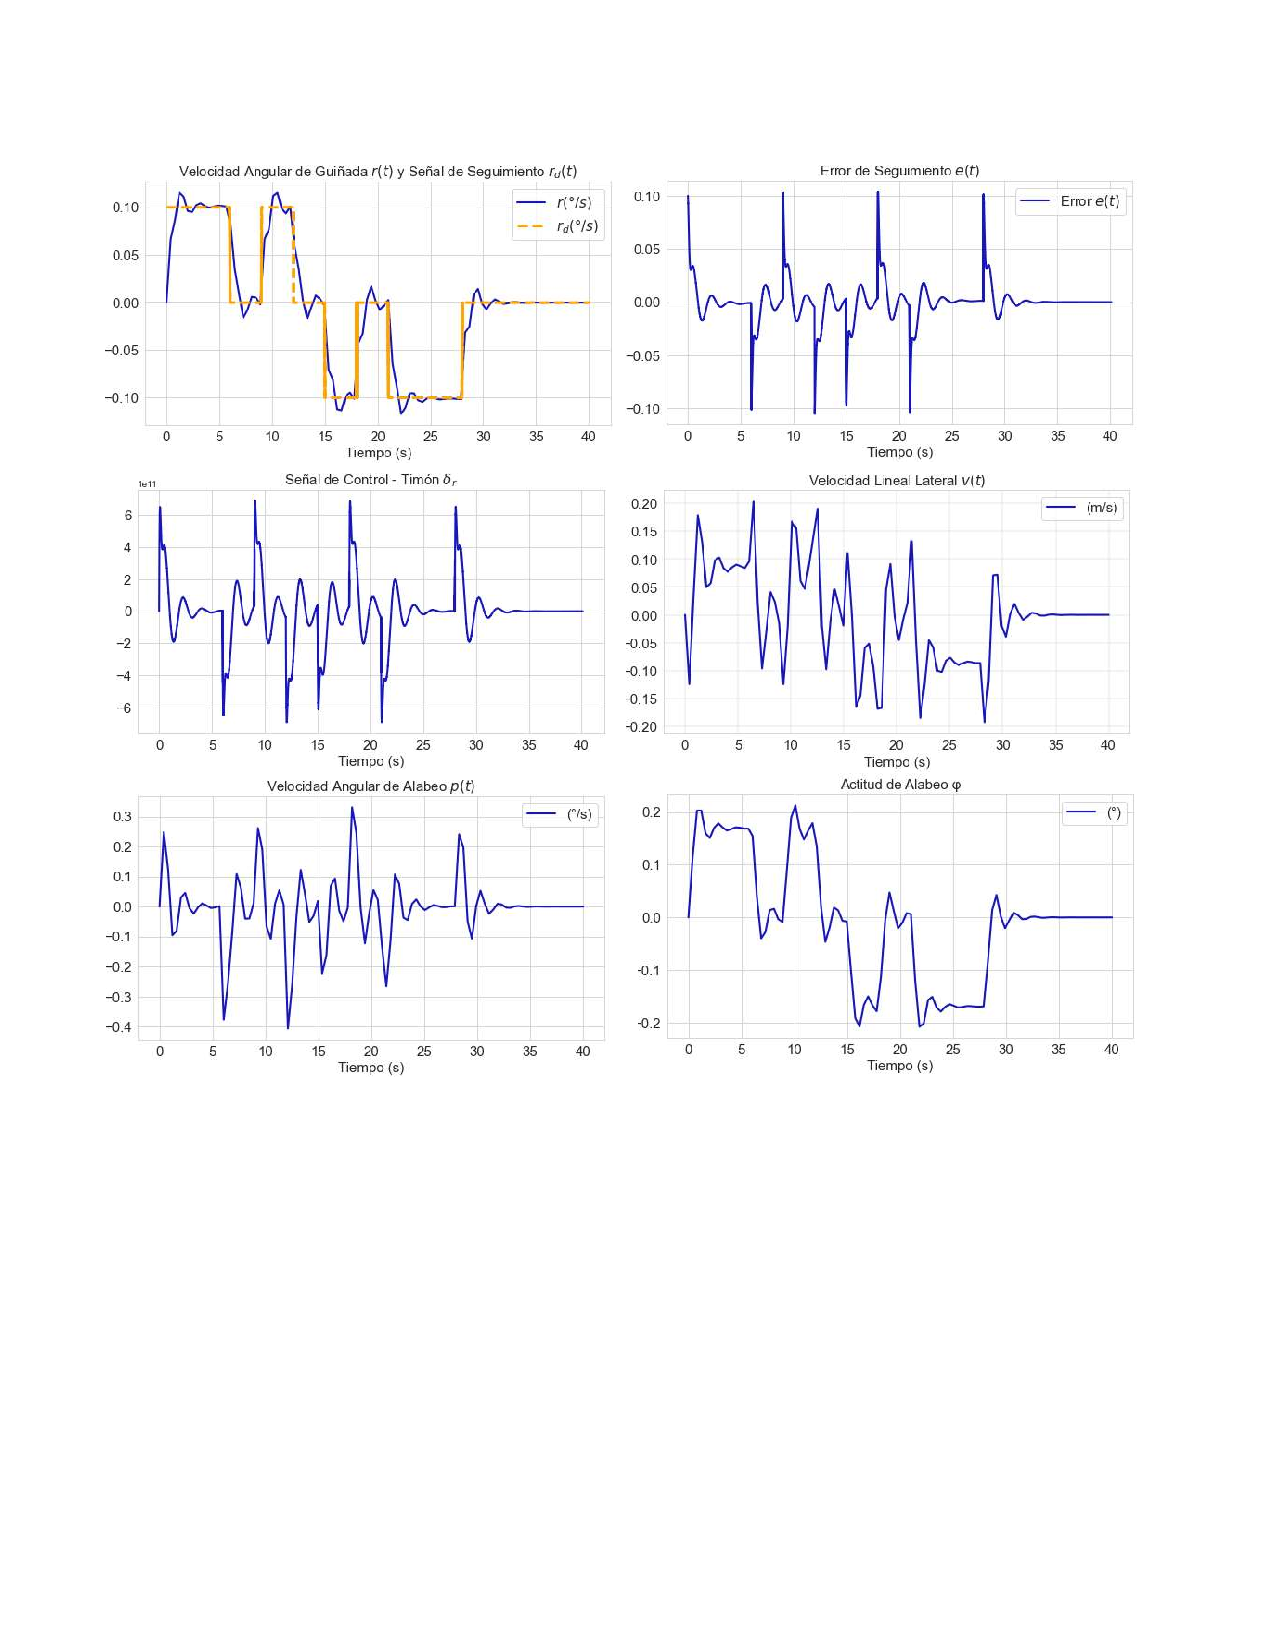
\includegraphics[scale=0.78]{Capitulo3/figs/Simulacion PID direccional_cropped.pdf}
    \caption{Simulation with Directional PID Controller}
    \label{Simulación de Giro Direccional con Controlador PID}
\end{figure}

\begin{table}[!h]
    \centering
    \begin{tabular}{|c|c|}
    \hline
    \multicolumn{2}{|c|}{PID Controller Gains}\\
    \hline
     Proportional $k_p$ & $-1377938545499.12$ \\
     Integral $k_i$ & $-616745432554.002$\\
     Derivative $k_d$ & $17142526949.4437$\\
     \hline
    \end{tabular}
    \caption{Directional PID Controller Gains}
    \label{Ganancias del Controlador PID direccional}
\end{table}

\textbf{Discussion of the Results.} Figure \ref{Simulación de Giro Direccional con Controlador PID} displays the PID directional controller simulations for EHEKATL BWB. 
%
In graph (a) it is perceived that the directional PID controller is less robust than the longitudinal and lateral PID controllers, showing oscillations for the signal approach $r(t)$ to the follow-up signal $r_d(t)$. However, this behavior also coincides with the actual physical sense, since the yaw movement is difficult to maintain due to the symmetry of the aircraft, and this oscillatory movement around a desired path in the course or direction is normal in fixed wing aircraft. 
 %
 In graph b) we have the tracking error $e(t)$. Unlike previous errors (longitudinal and lateral dynamics) here the $e(t)$ shows oscillatory and smoother behavior. 
 %
 Figure (c) shows the control signal of steering rudders $\delta_r$. The control signal is too large, it is in order 1e11. This huge result of $\delta_r$ is due to the values so small that they were obtained in the control vector $B$ of the equation \ref{direcciooal lineal EHEKATL BWB}. For the same reason the gains of the Table \ref{Ganancias del Controlador PID direccional} They're so big. 
 %
 In graph d) the linear lateral velocity is shown $v(t)$. This graph goes in the same direction as the tracking signal $r_d(t)$ but with a range of $-0.2 m/s$ and $0.2 m/s$. 
 %
 Figure (e) shows the angular wing speed $p(t)$, with an answer between $-0.4m/s$ and $0.3m/s$. 
 %
 Figure (f) shows the attitude of roll $\phi(t)$. The answer coincides with the $r_d(t)$ in the sense, where positive is direction to the right and negative direction to the left. 

PID controllers designed for EHEKATL BWB can be used for applications similar to those NASA had with its X-48 B/C wing-integrated aircraft, where independent PID controllers were deployed for pitching, rolling and yawing moments.
%
During the simulation process with the PID controllers it was observed that with new tracking signals (sine-like or pass-through type but with more complex functions) it is necessary to re-tune the gains. Re-adjustment of gains is mainly due to the fact that simulations are invariant over time. Important consideration to have, since the actual application of the controllers will be for time-variant systems, this exercise is a first control approach for the applications shown in the chapter of \textit{EHEKATL BWB flight simulations}.  


%%%%%%%%%%%%%%%%%%%%%%%%%%%%%%%%%%%%%%%%%%

%%%%%%%%%%%%%
\section{Linear Quadratic Regulator}

The Linear Quadratic Regulatory Control\footnote{Linear Quadratic Regulator, or LQR} is an advanced control technique used in linear dynamic systems. 
%
Your goal is to design a controller that minimizes a quadratic cost function.
%
The LQR control is based on two key aspects: the formulation of a quadratic cost function that quantifies the desired performance of the system and the resolution of the Riccati equation to obtain the driver gains that minimize this cost function. 
%
Recalling the dynamic model chapter, for the LQR controller we use the EHEKATL BWB system in state space given the shape $\dot x = Ax + Bu$, where $x$ is the vector of states and $u$ is the vector of control inputs. 

The aim is to minimize a quadratic cost function defined as:
\begin{equation}
    J = \int_0^{\infty} (x^T Qx + u^T Ru) dt
\end{equation}
where Q and R are the weighting matrices that determine the relative importance of states and control inputs in the total cost.

The Riccati equation in the LQR controller is a matrix equation that is used to find the optimal winning matrix $K$ The equation is as follows:
\begin{equation}
    A^T P + P A - P B R^{-1} B^T P + Q = 0
\end{equation}
where $A$ is the matrix of states of the system, $B$ is the input matrix of the system, $R$ is the weighting matrix of the control entries, $Q$ is the weighting matrix of the states and $P$ It's the solution matrix we're looking for. 

To apply the LQR Control, you must first have the system model in the form of state space with the matrices $A$ and $B$ defined.
%
Subsequently, Q and R weighting matrices based on control objectives are chosen. Choosing these matrices will affect controller performance. 
%
The Riccati equation is a quadratic equation in $P$, and can be solved in various ways depending on the nature of the matrices involved. The solution can be analytical or numerical. In practice, it is common to use computational tools to find the numerical solution to the Riccati equation. 
%
The library is used \textit{control.matlab} for Python to estimate $P$. The matrix $P$ contains information on how system states and control inputs are related to minimize quadratic cost function. 
%
The solution of the Riccati equation provides optimal gains for the LQR controller, which means that the resulting controller will minimize the quadratic cost function.
%
It is important to note that the Riccati equation can have multiple solutions. In practice, the solution will depend on the specific objectives of the controller design. 

\medskip

\textbf{Simulation of LQR Control for Cruise Flight}\\
Like the previous PID controller, LQR uses the linear system with time-invariant parameters. 
%
\begin{figure}[!t]
    \centering
    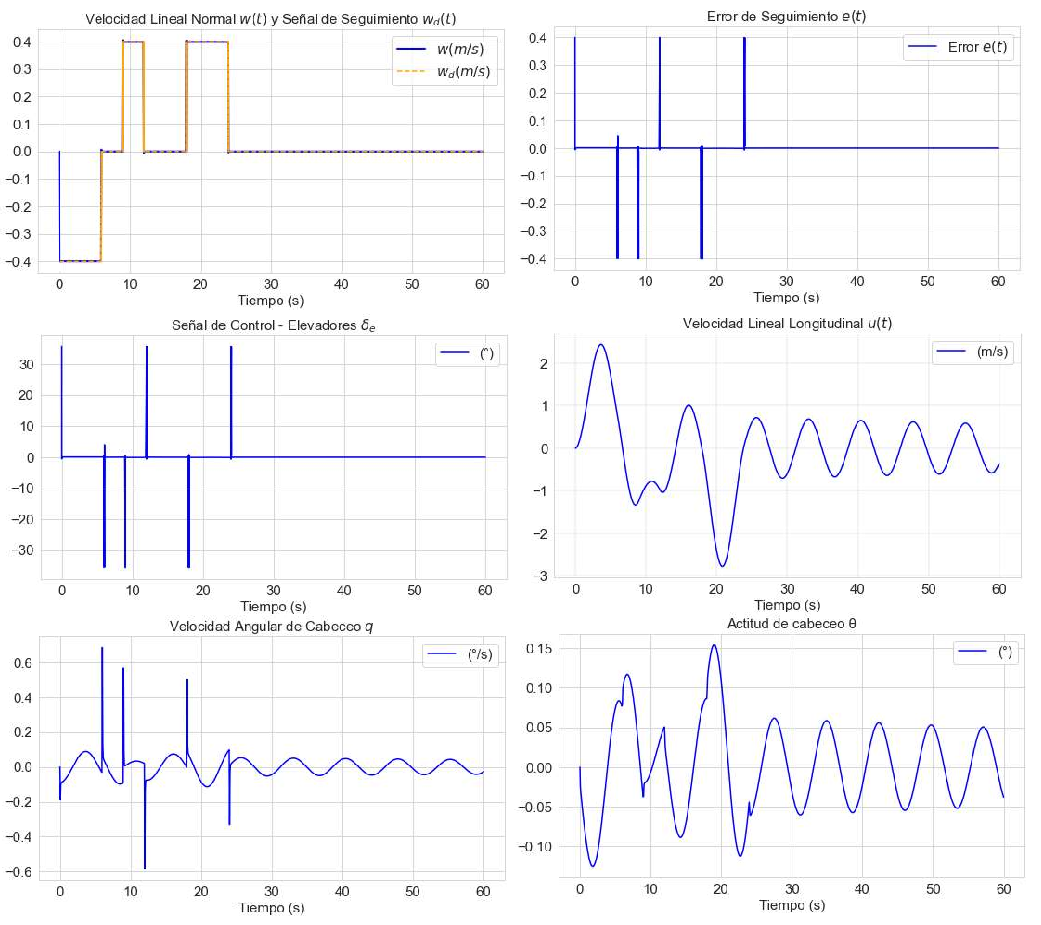
\includegraphics[scale=0.8]{Capitulo3/figs/LQR longitudinal.pdf}
    \caption{Simulation with LQR Controller for EHKATL BWB Cruise Flight}
    \label{Simulación con Controlador LQR para Vuelo Crucero de EHKATL BWB}
\end{figure}
The values of EHEKATL BWB system A and B are shown. 
\begin{equation}
    \begin{bmatrix}
    \dot u \\
    \dot w \\
    \dot q \\
    \dot \theta
    \end{bmatrix}
    =
    \begin{bmatrix}
    -0.0276445 & 0.467688 & 0 & -9.81 \\
    -1.1998 & -6.03618 & 13.3267 & 0 \\
    -6.70053e-07 &-4.84984 & -6.13596 & 0 \\
    0 & 0 & 1 & 0 \\ 
    \end{bmatrix}
        \begin{bmatrix}
    u \\
    w \\
    q \\
    \theta
    \end{bmatrix}
    +
    \begin{bmatrix}
    0.4311744\\
    -13.21339\\
    -27.35091\\
    0\\
    \end{bmatrix}
    \delta_{e}
\end{equation}

The values of the proposed Q and R weighting matrices for longitudinal dynamics are shown. 
\begin{equation}
Q
=
\begin{bmatrix}
6 & 0 & 0 & 0 \\
0 & 18 & 0 & 0 \\
0 & 0 & 3 & 0 \\
0 & 0 & 0 & 0.1
\end{bmatrix} 
\quad
    R
    =
    \begin{bmatrix}
    0 & 0 & 0 & 0 \\
    0 & 0.001 & 0 & 0  \\
    0 & 0 & 0 & 0 \\
    0 & 0 & 0 & 0 \\
    \end{bmatrix}
\end{equation}

And according to the dynamic system of EHEKATL BWB for an instant in time (invariant in time) described by the A and B matrices, and our weighting in the Q and R matrices, we calculate numerically through the library of $control.matlab$ in Python gains from the controller matrix $k$.
\begin{equation}
    K
    =
    \begin{bmatrix}
    48.9349891 & -89.19222159 & -41.54753902 & -691.77049282 \\
    \end{bmatrix}
\end{equation}
Figure \ref{Simulación con Controlador LQR para Vuelo Crucero de EHKATL BWB} shows the results obtained after applying the same reference signal to the LQR controller $w_d$ that we apply to the PID controller. 
%
The results obtained with the LQR controller are very similar to those obtained with the PID controller, which was of course expected given the same follow-up signal $w_d$ and share values in A and B. 

\medskip

%%%%%%%%%%%%%%%%%%
\textbf{LQR Control Simulation for Lateral Spin}\\
The linear dynamic system invariant in time is used for lateral dynamics, see equation \ref{lateral lineal LQR EHEKATL BWB}. Figure \ref{Simulación con Control LQR para la dinámica lateral de EHEKATL BWB} displays the simulations with the LQR controller for EHEKATL BWB assuming a sustained lateral rotation at constant speed. 
\begin{figure}[!h]
    \centering
    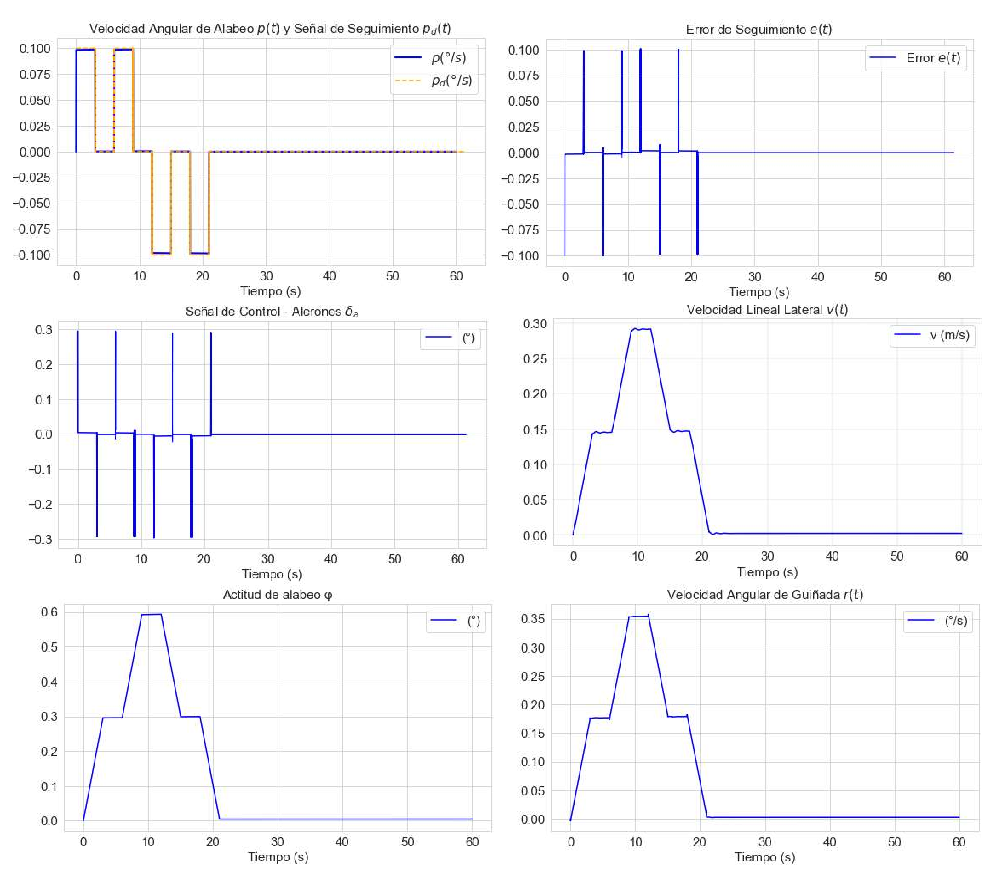
\includegraphics[scale=0.75]{Capitulo3/figs/LQR lateral.pdf}
    \caption{Simulation with LQR control for EHEKATL BWB lateral dynamics}
    \label{Simulación con Control LQR para la dinámica lateral de EHEKATL BWB}
\end{figure}
\begin{equation}
\label{lateral lineal LQR EHEKATL BWB}
    \begin{bmatrix}
        \dot v \\
        \dot p \\
        \dot r \\
        \dot \phi
    \end{bmatrix}
    =
    \begin{bmatrix}
    -0.440144 & -0.263171 & -16.0681 & 9.81 \\
    -8.22254 & -22.4261 & 8.34045 & 0 \\
    2.0262 & 1.4176 &-1.72499 & 0 \\
    0 & 1 & 0 & 0 \\
    \end{bmatrix}
    \begin{bmatrix}
        v \\
        p \\
        r \\
        \phi
    \end{bmatrix}
    +
    \begin{bmatrix}
    2.882972 \\
    500.764 \\
    -18.97689 \\
    0\\
    \end{bmatrix}
    \delta_a
\end{equation}
The weighting of profit Q and R is proposed. 
\begin{equation}
Q
=
\begin{bmatrix}
3 & 0 & 0 & 0 \\
0 & 9 & 0 & 0 \\
0 & 0 & 9 & 0 \\
0 & 0 & 0 & 3
\end{bmatrix} 
\quad
R
=
\begin{bmatrix}
0 & 0 & 0 & 0 \\
0 & 1 & 0 & 0  \\
 0 & 0 & 0 & 0 \\
0 & 0 & 0 & 0 \\
\end{bmatrix}
\end{equation}

and according to the parameterization of A,B,Q,R the gains of the controller are obtained by means of numerical methods solution $k$.
\begin{equation}
    K
    =
    \begin{bmatrix}
     0.11366923 &  2.95176288 & -0.16714788 &   2.67770629\\
    \end{bmatrix}
\end{equation}
The proposal for relative weighting proposed by a server in the Q and R matrices resulted in excellent results for controlling lateral dynamics using LQR. 

%%%%%%%%%%%%%%%%%%
\section{Python Codes}
\label{a codigos python}
The codes developed in this thesis project are shared in the Git-Hub personal account of the thesis author. Here is the access: 
\href{https://github.com/Galexs-Aerospace/Aircraft-Design-and-Control.git}{Aircraft Design and Control} o si prefiere: https://github.com/Galexs-Aerospace/Aircraft-Design-and-Control.git
